\documentclass{article}

\usepackage{graphicx}

\usepackage[margin=0.5cm]{geometry}
\usepackage{amsmath}
\usepackage{indentfirst}
\usepackage{hyperref}
\usepackage{multirow}
\usepackage{comment}

\newcommand{\cosa}{\cos\hat\alpha}
\newcommand{\size}{0.33\textwidth}
\newcommand{\pt}{p_\text{T}}

\begin{document}

\title{Data vs MC comparison for 8 and 13 TeV $Z$ using LO PDFs}
\author{Mariana Ara\'ujo (LIP)}
\maketitle

\section{Procedure}

\begin{itemize}
\item The MC distributions are obtained by filling a $\xi$ histogram with events within the fiducial cuts determined for each data measurement. 
\item The weights are those determined in the MC generation, from the Z production cross-section formula with the assumption of transverse polarization in the ppHX frame, and the Jacobian factor. 
\item All distributions are then scaled by the same factor (currently $40$) to match up with data. No $\sqrt{s}$-based scaling factor is added, such as based on the number of events in the sample or on the sum of all Jacobian factors. 
\item The 8 TeV ATLAS data, previously scaled up by a factor of 2 that we thought was missing in the corrections, is now back at its presented value, which fits well with the observed $\sqrt{s}$ scaling. It is the 8 TeV CMS data that now falls above the MC by a factor of almost exactly 2.
\end{itemize}

\clearpage

\newgeometry{margin = 0.5cm}

\begin{figure}[h!]
\centering
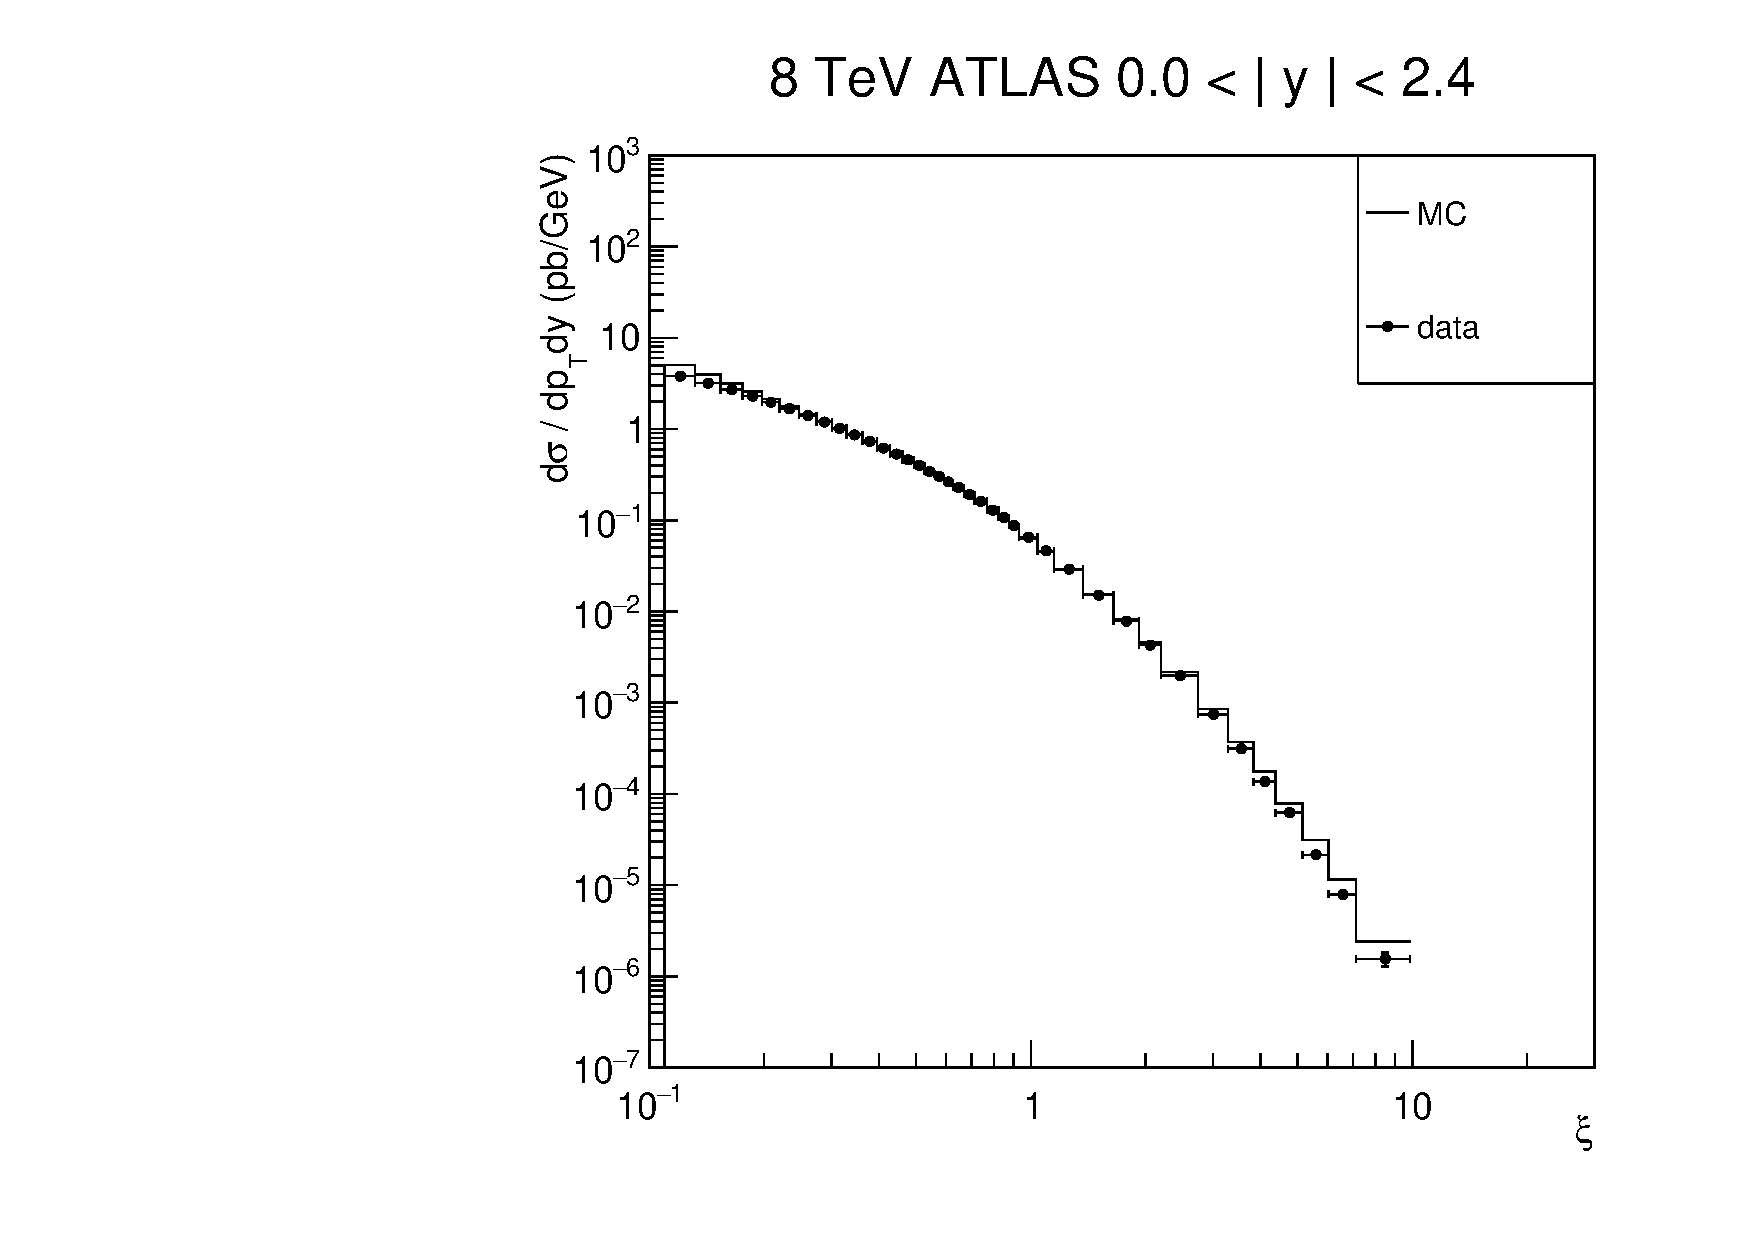
\includegraphics[width = 0.4\textwidth]{xi_8_A_y0.pdf}
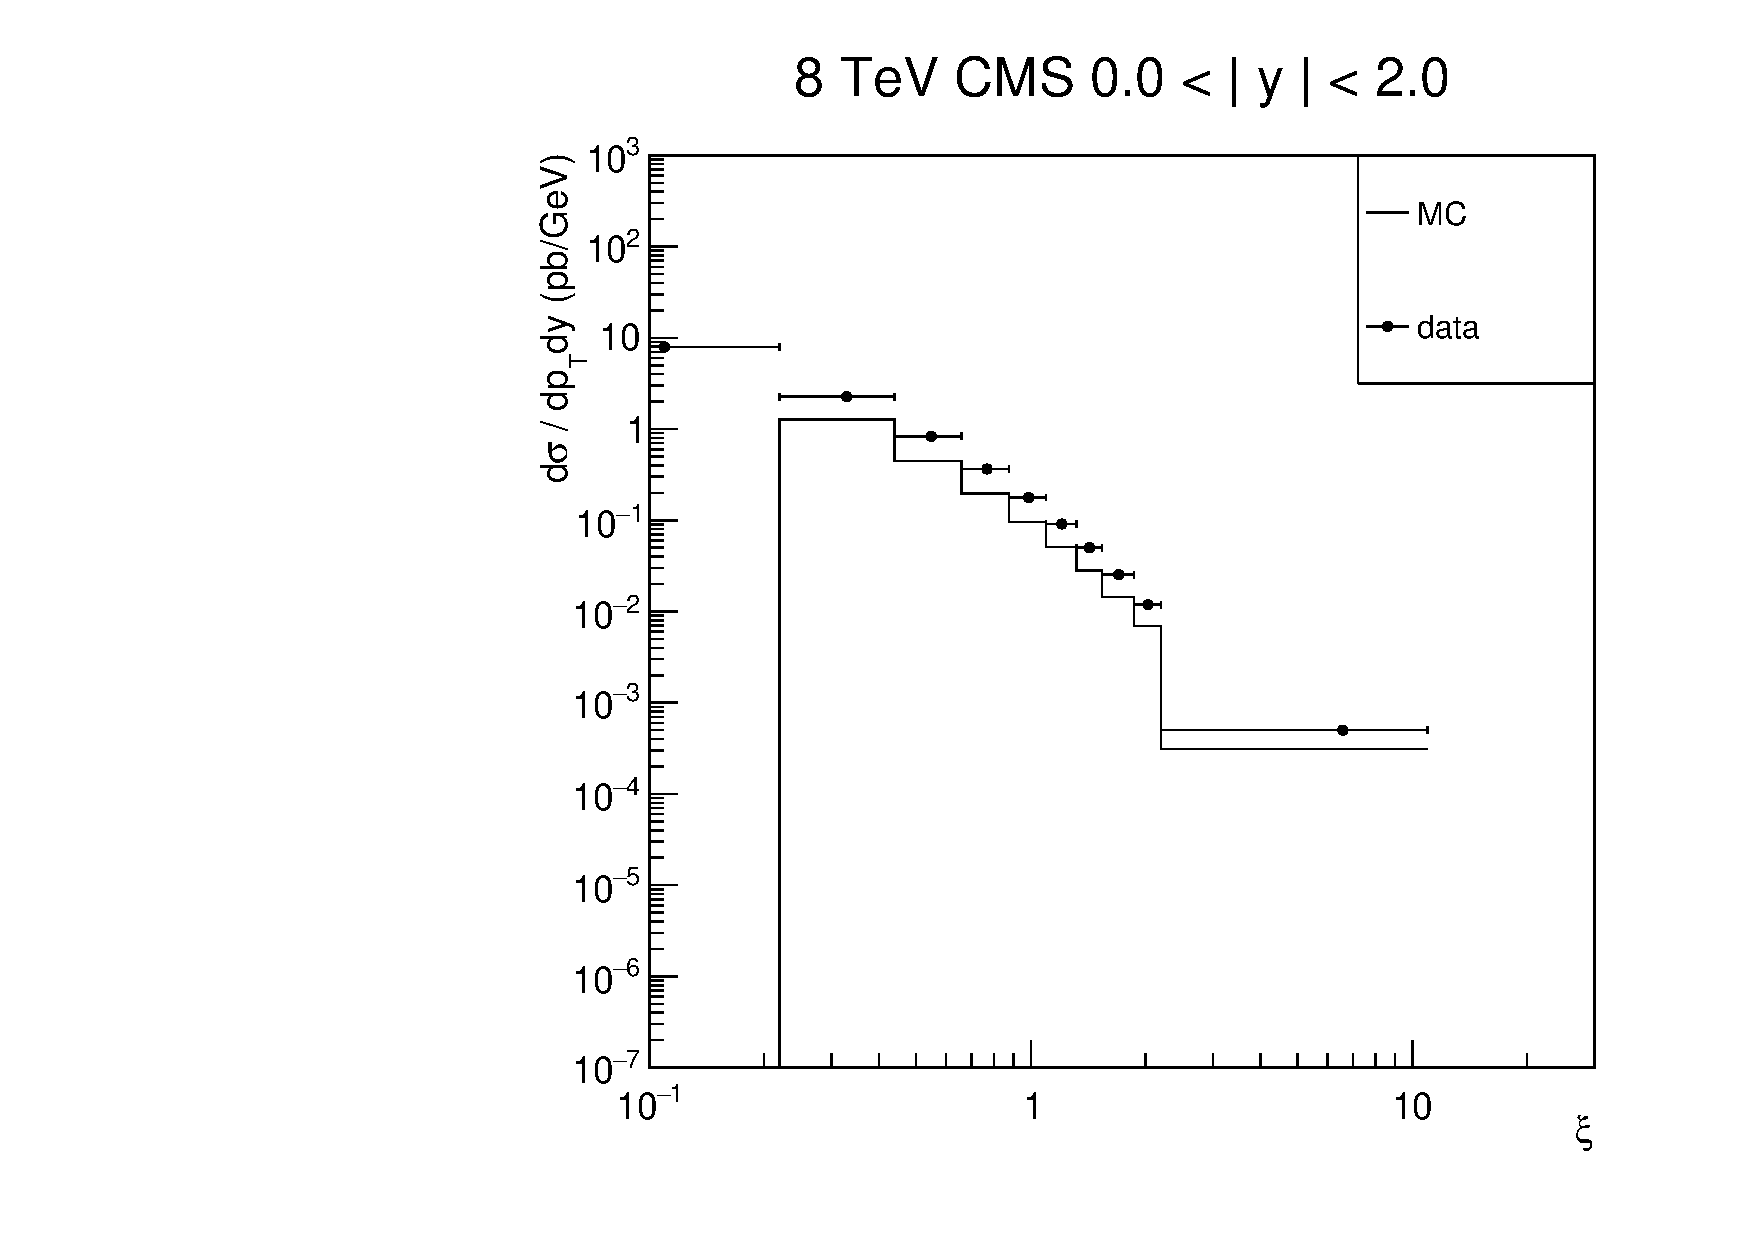
\includegraphics[width = 0.4\textwidth]{xi_8_C_y0.pdf}

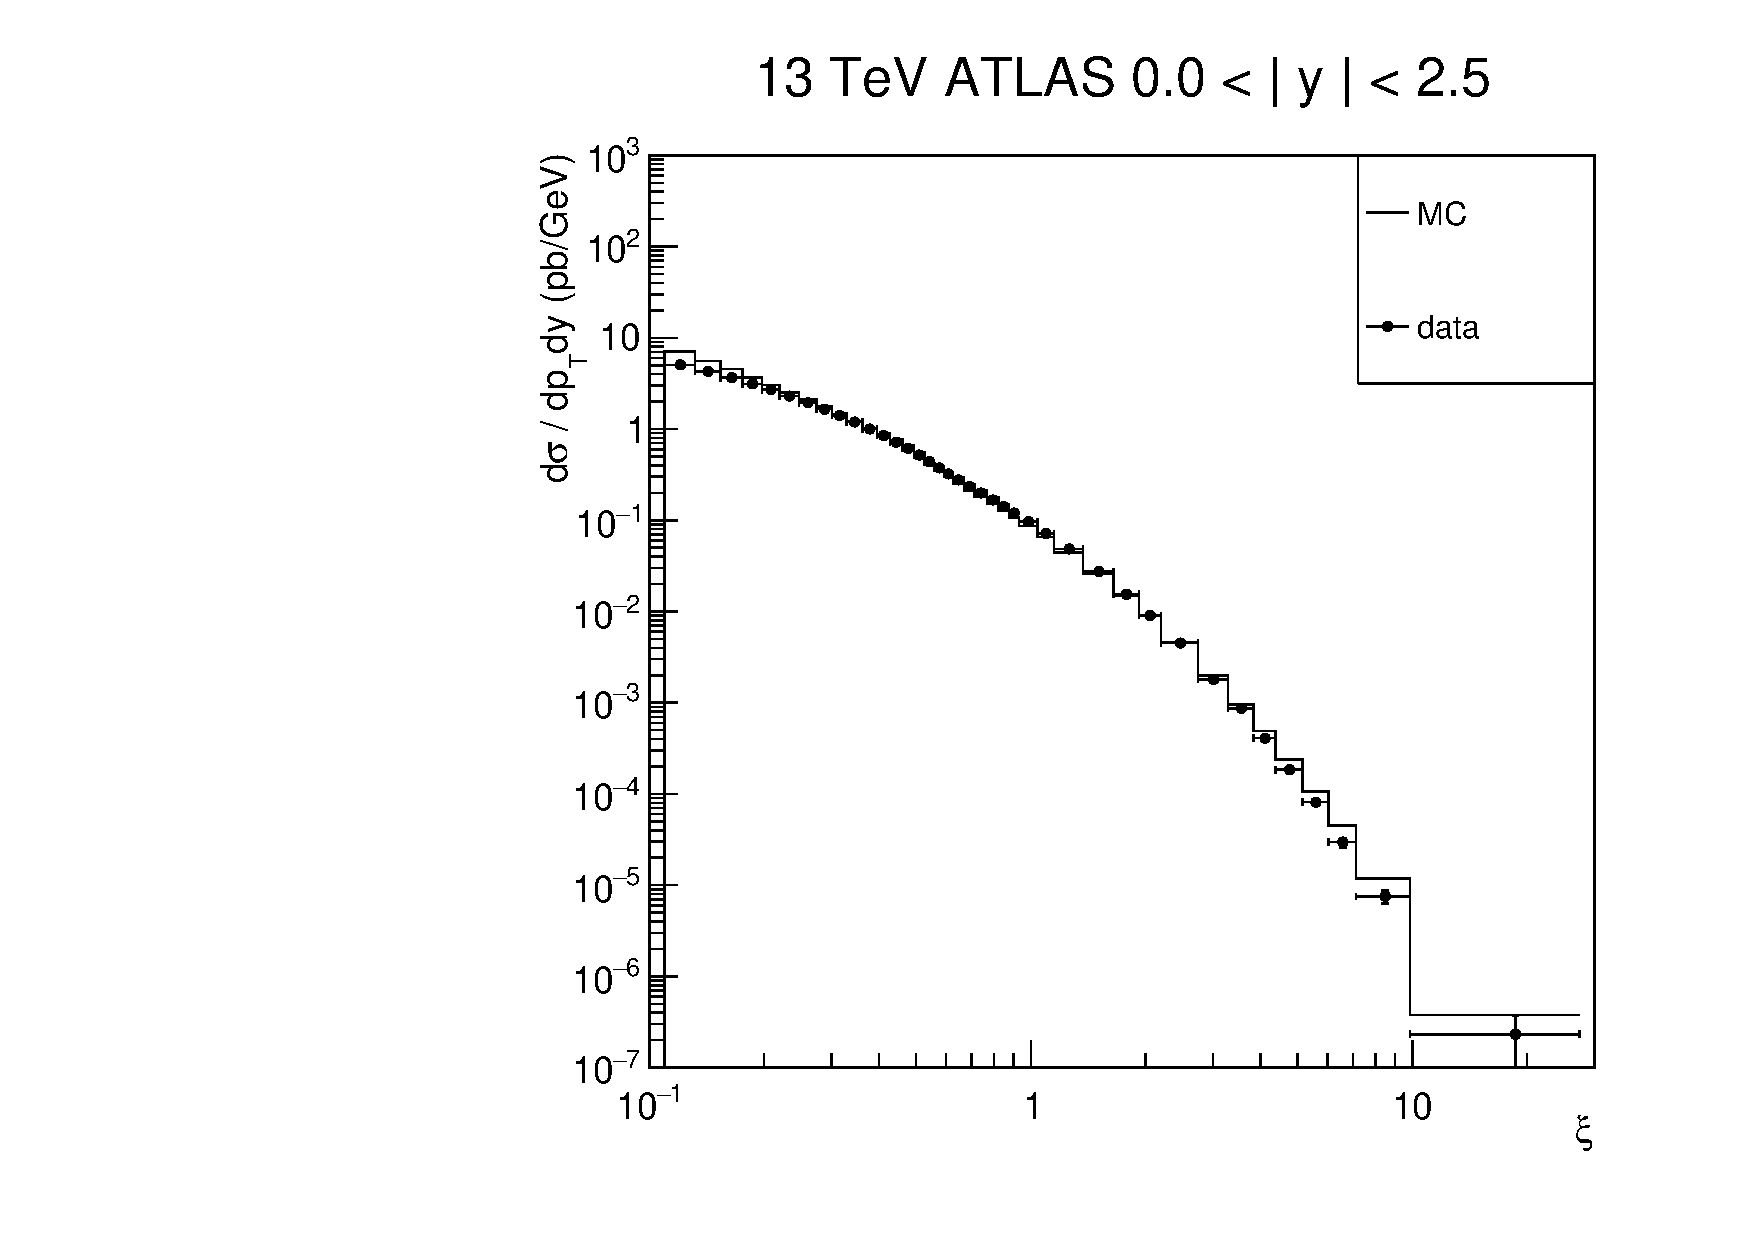
\includegraphics[width = 0.4\textwidth]{xi_13_A_y0.pdf}
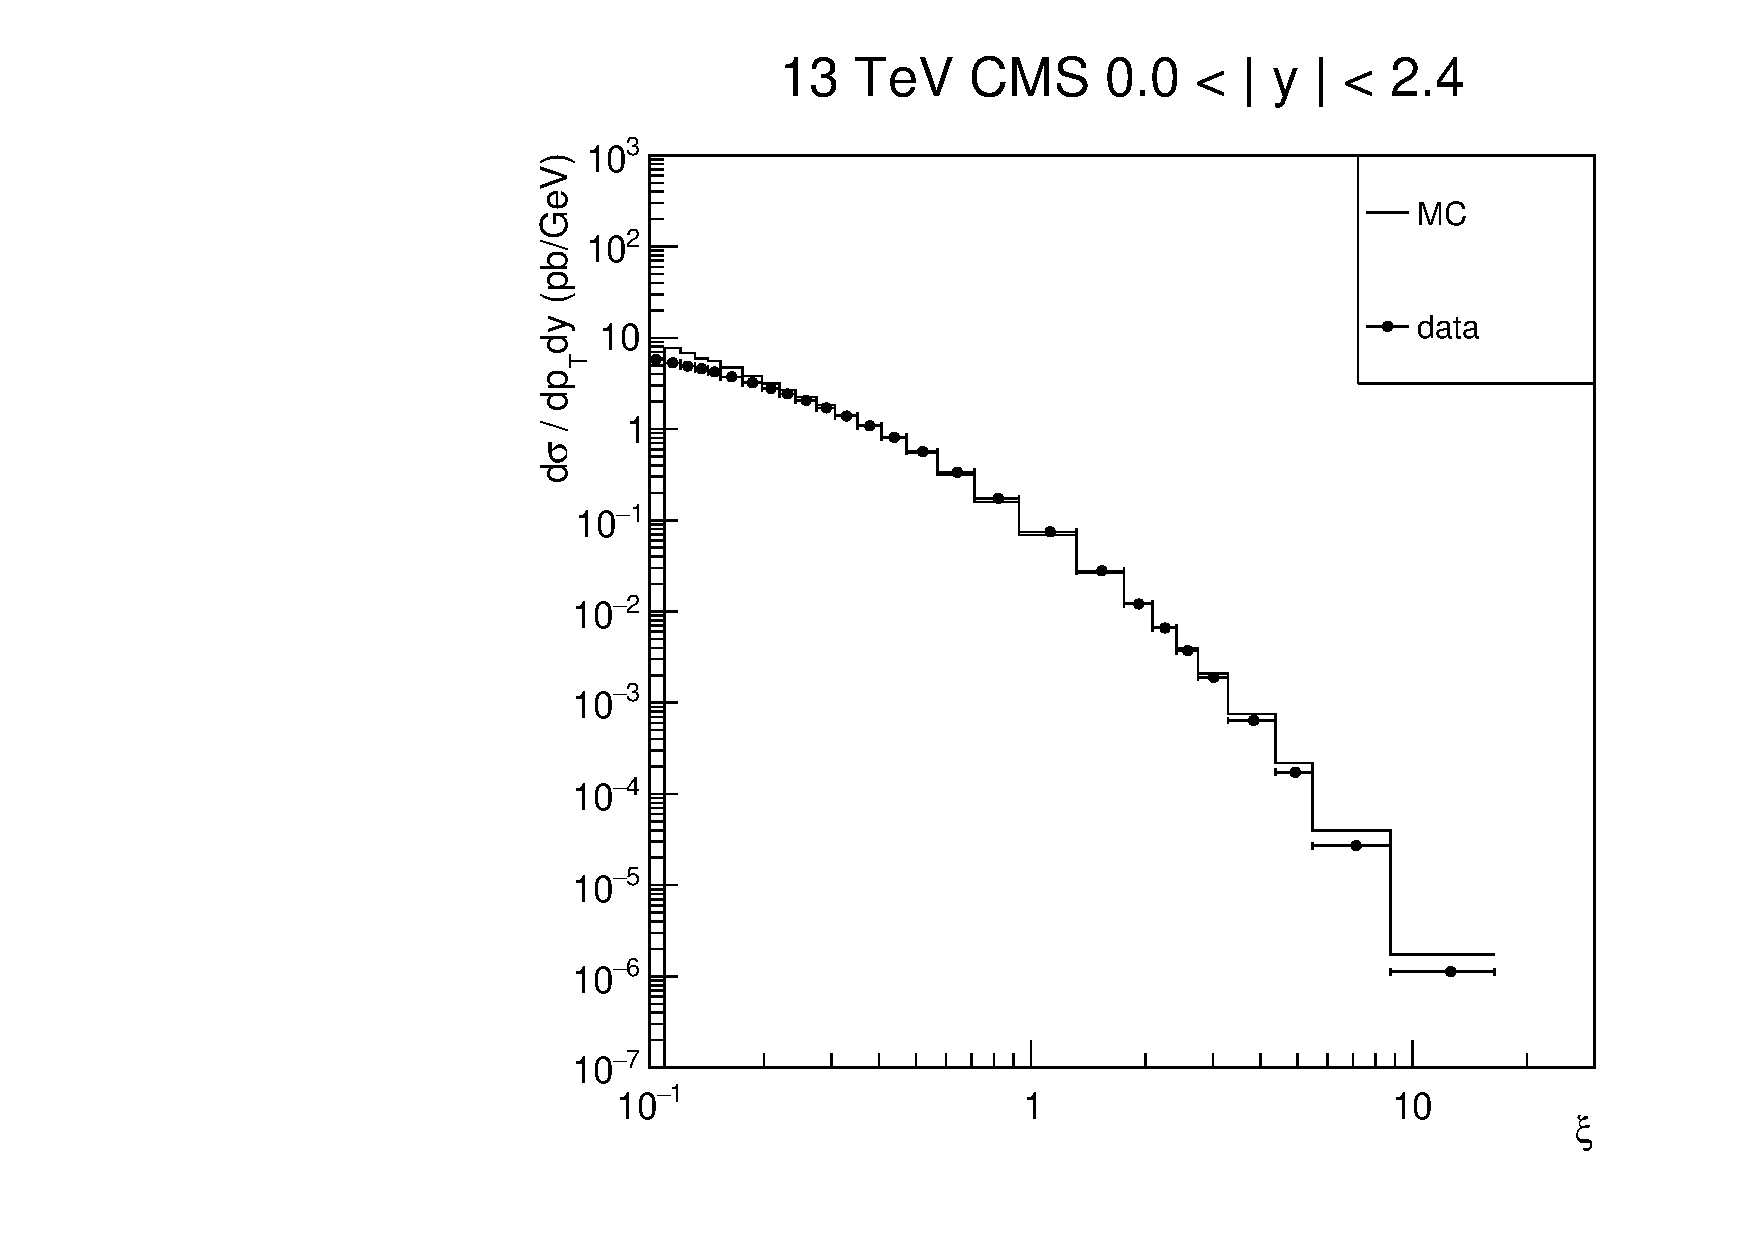
\includegraphics[width = 0.4\textwidth]{xi_13_C_y0.pdf}
%\caption{Comparison between MC $\xi$ distribution and data points in the six $y$ bins of the data, for 8 TeV. All histograms divided by total nr events and multiplied by same normalization factor. Data is not scaled.}\label{f:xi_comp}
\end{figure}

\clearpage

\begin{figure}[h!]
\centering
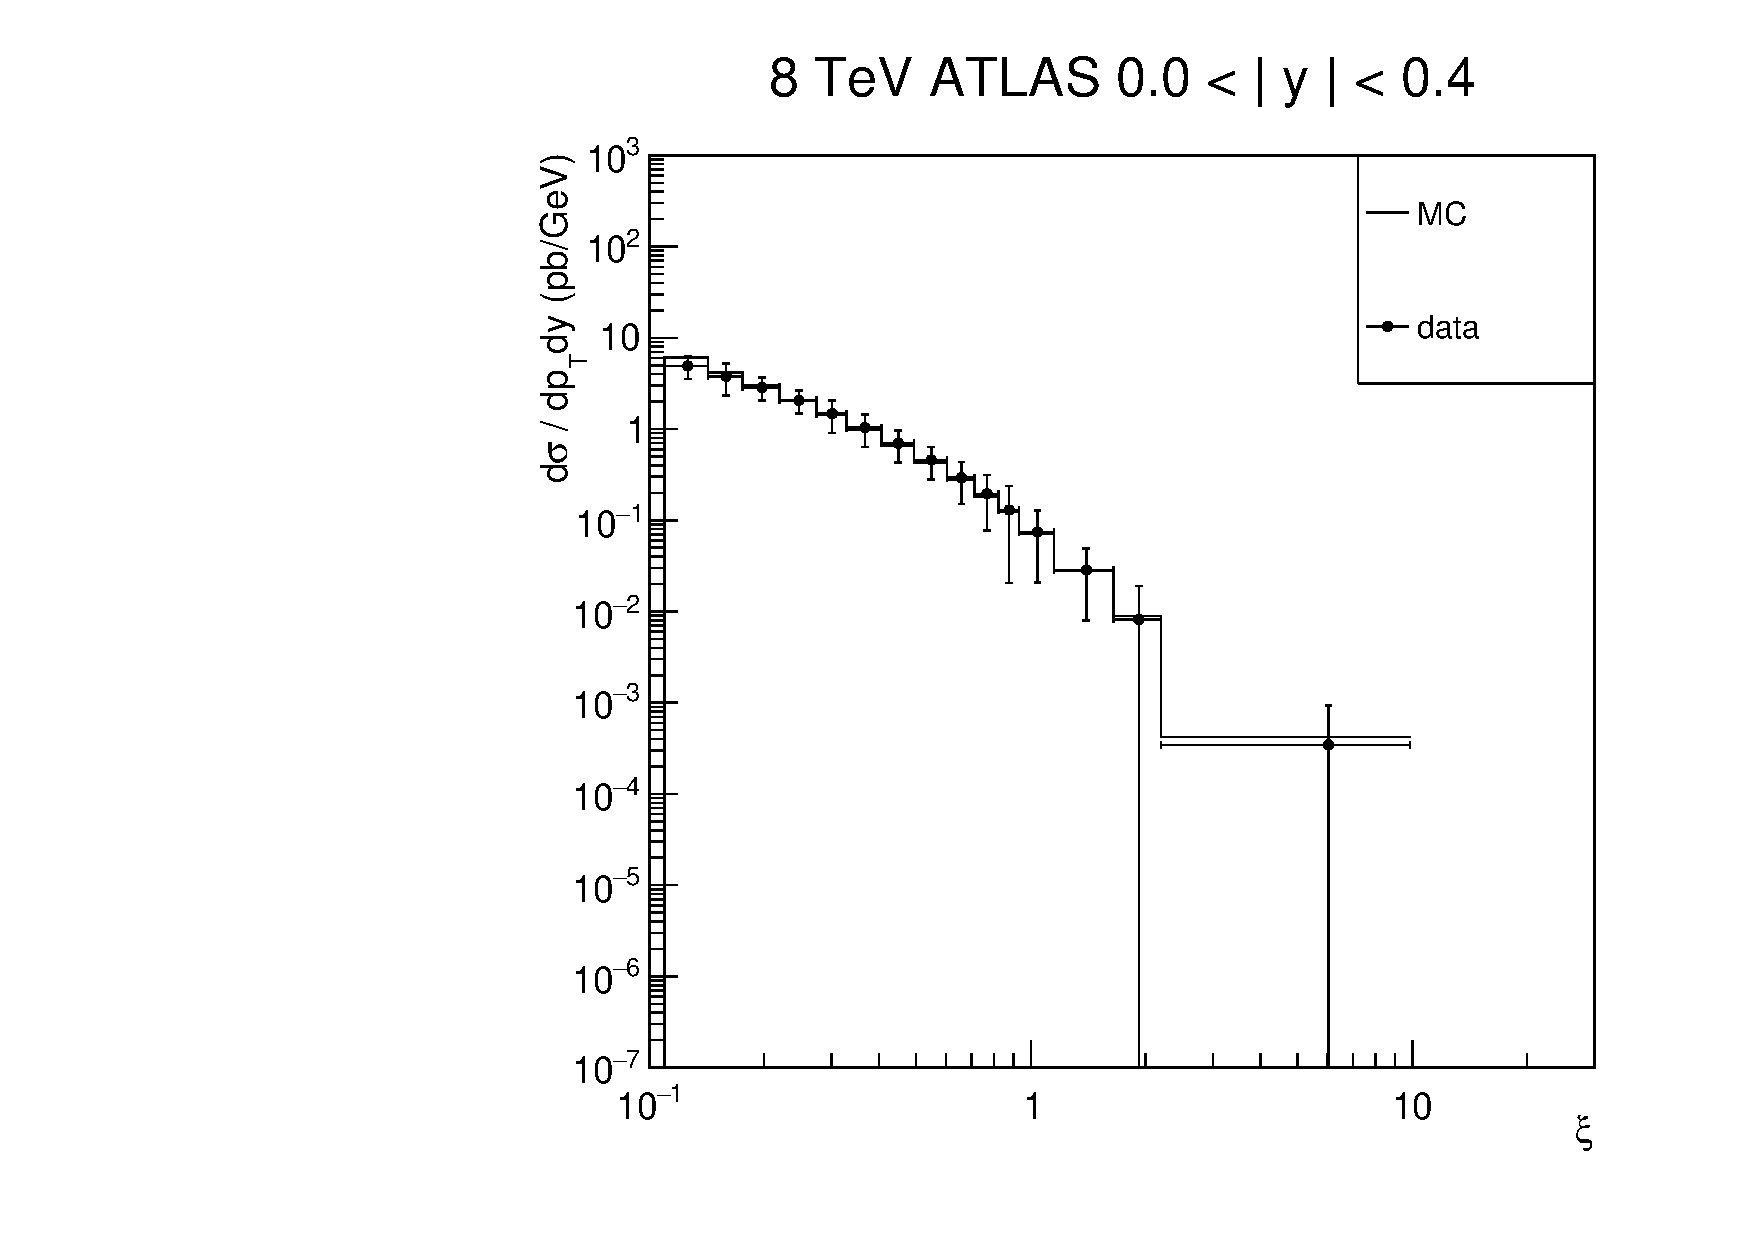
\includegraphics[width = 0.4\textwidth]{xi_8_A_y1.pdf}
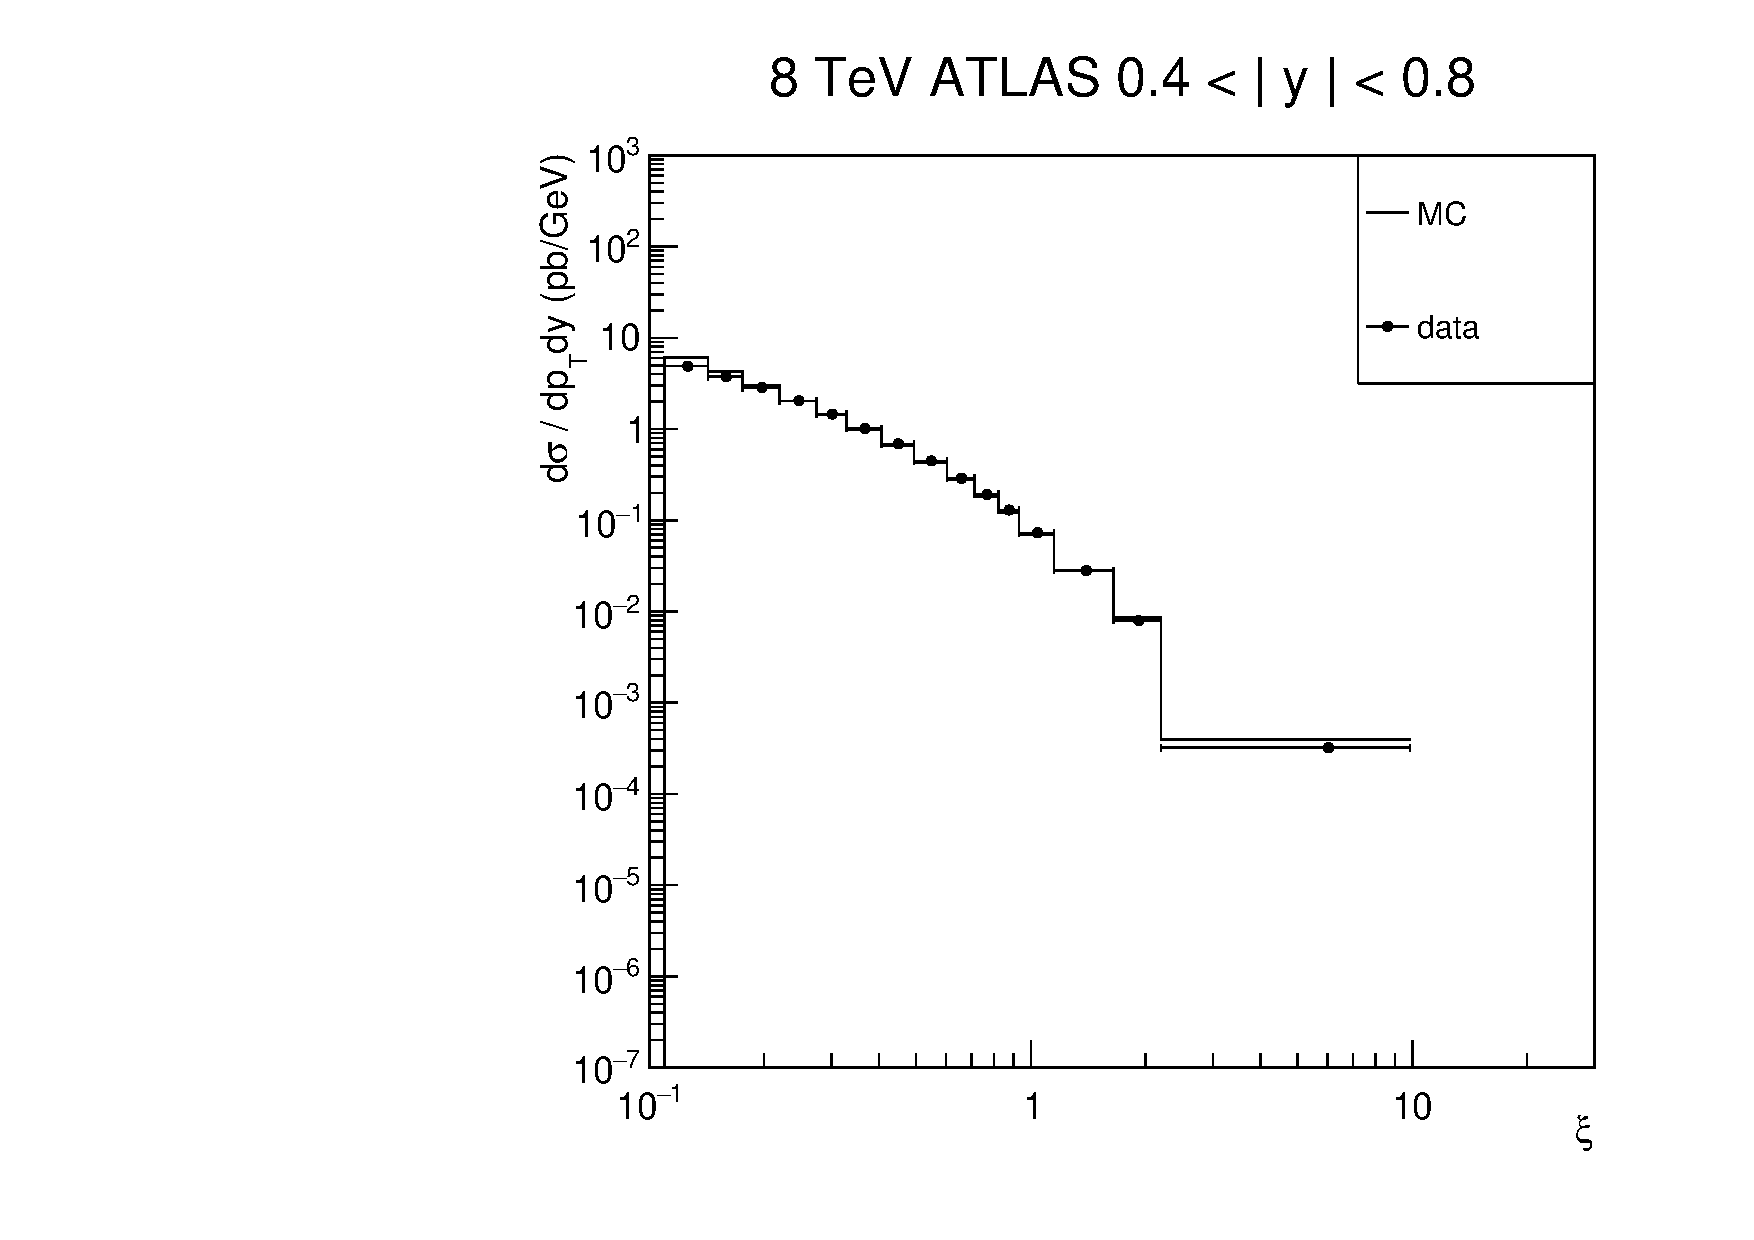
\includegraphics[width = 0.4\textwidth]{xi_8_A_y2.pdf}

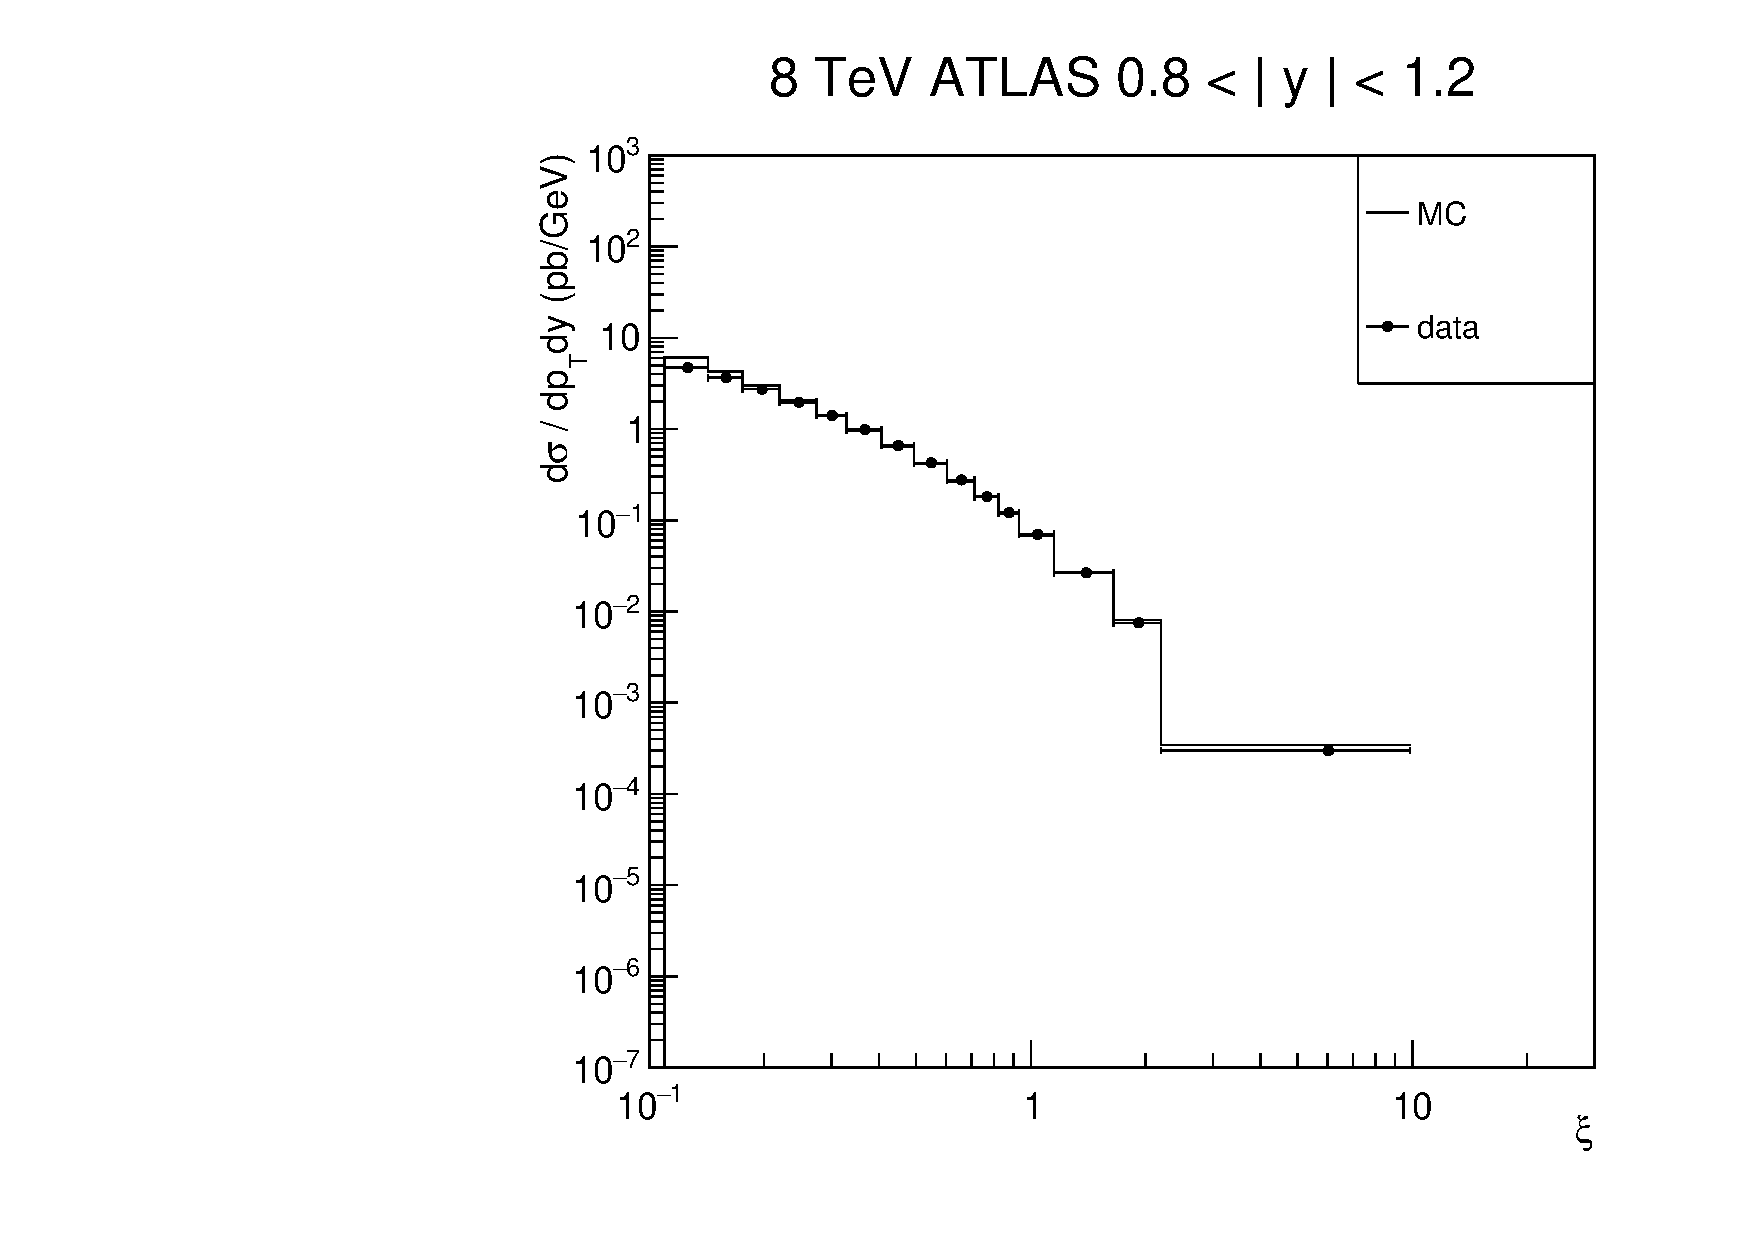
\includegraphics[width = 0.4\textwidth]{xi_8_A_y3.pdf}
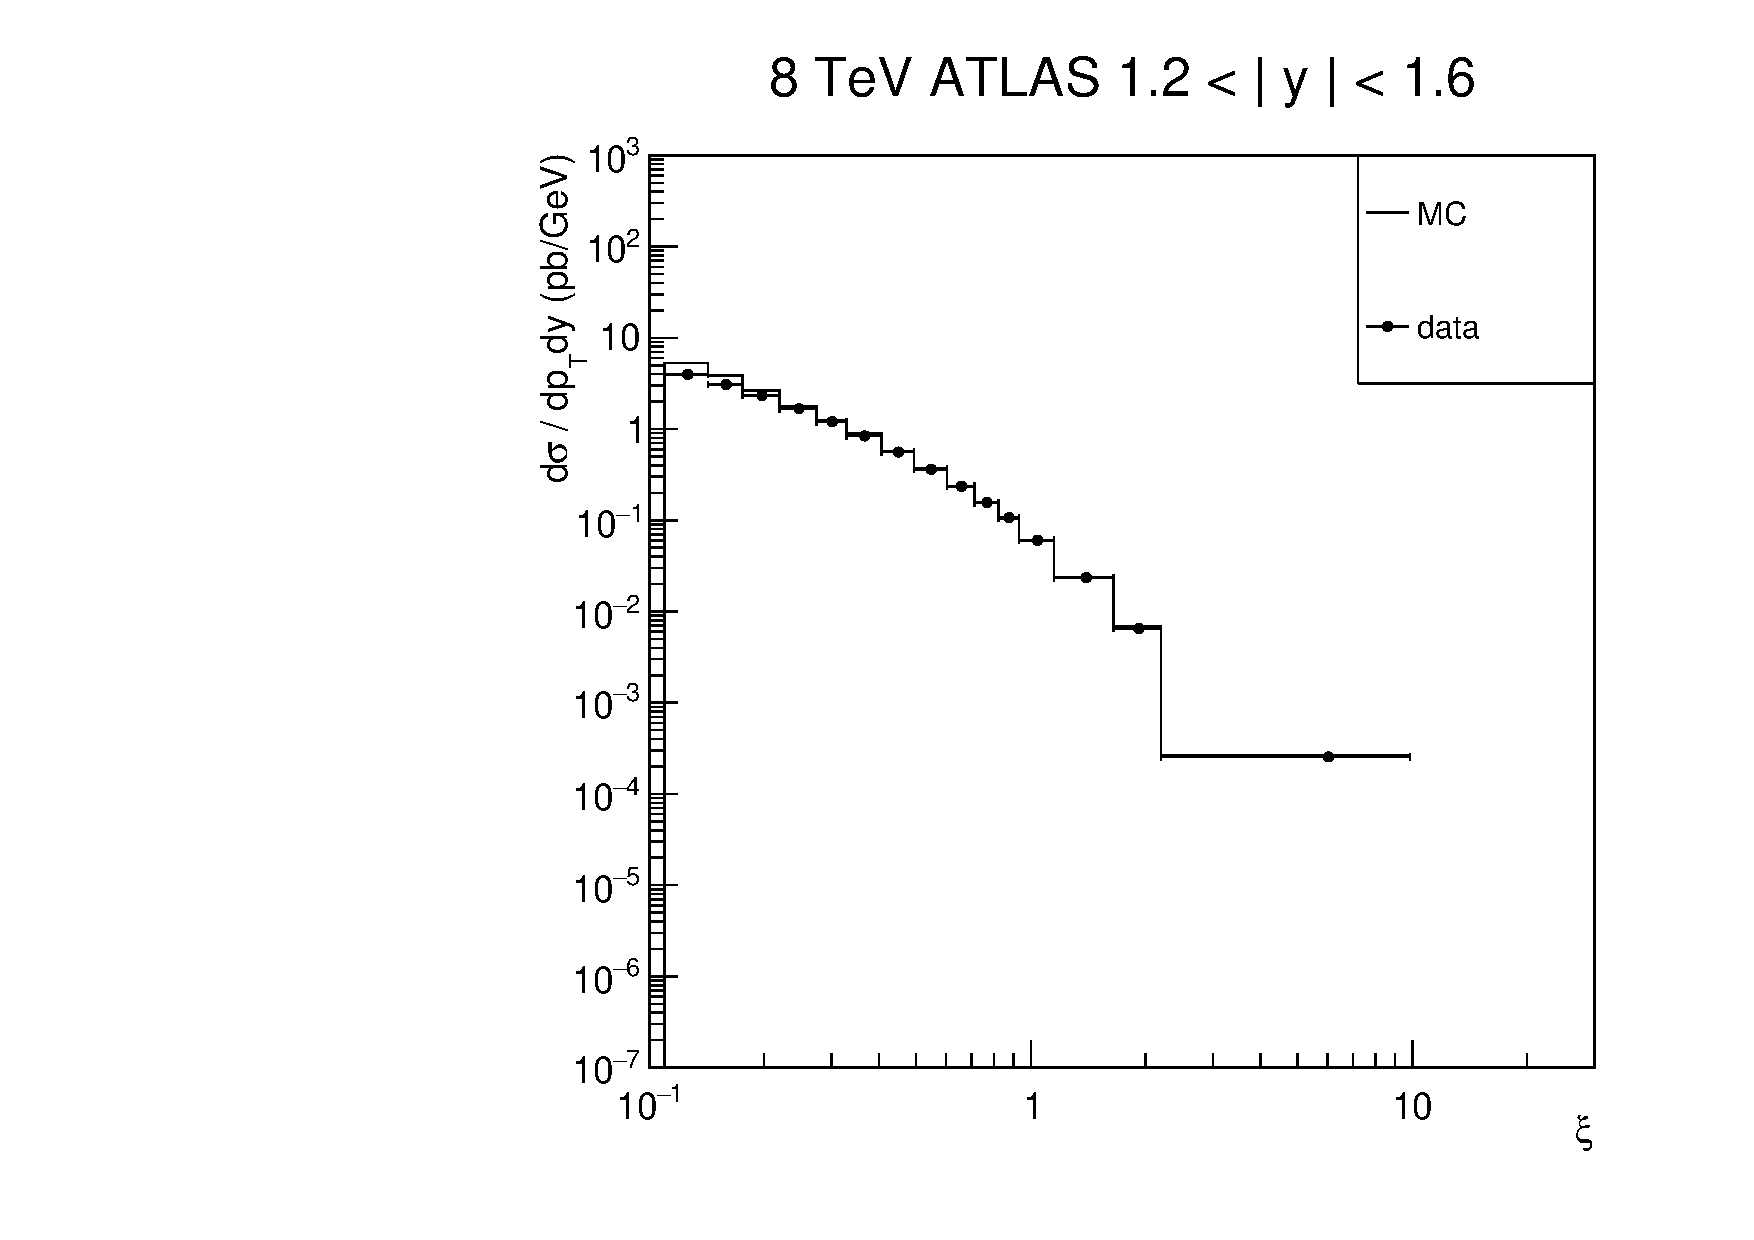
\includegraphics[width = 0.4\textwidth]{xi_8_A_y4.pdf}

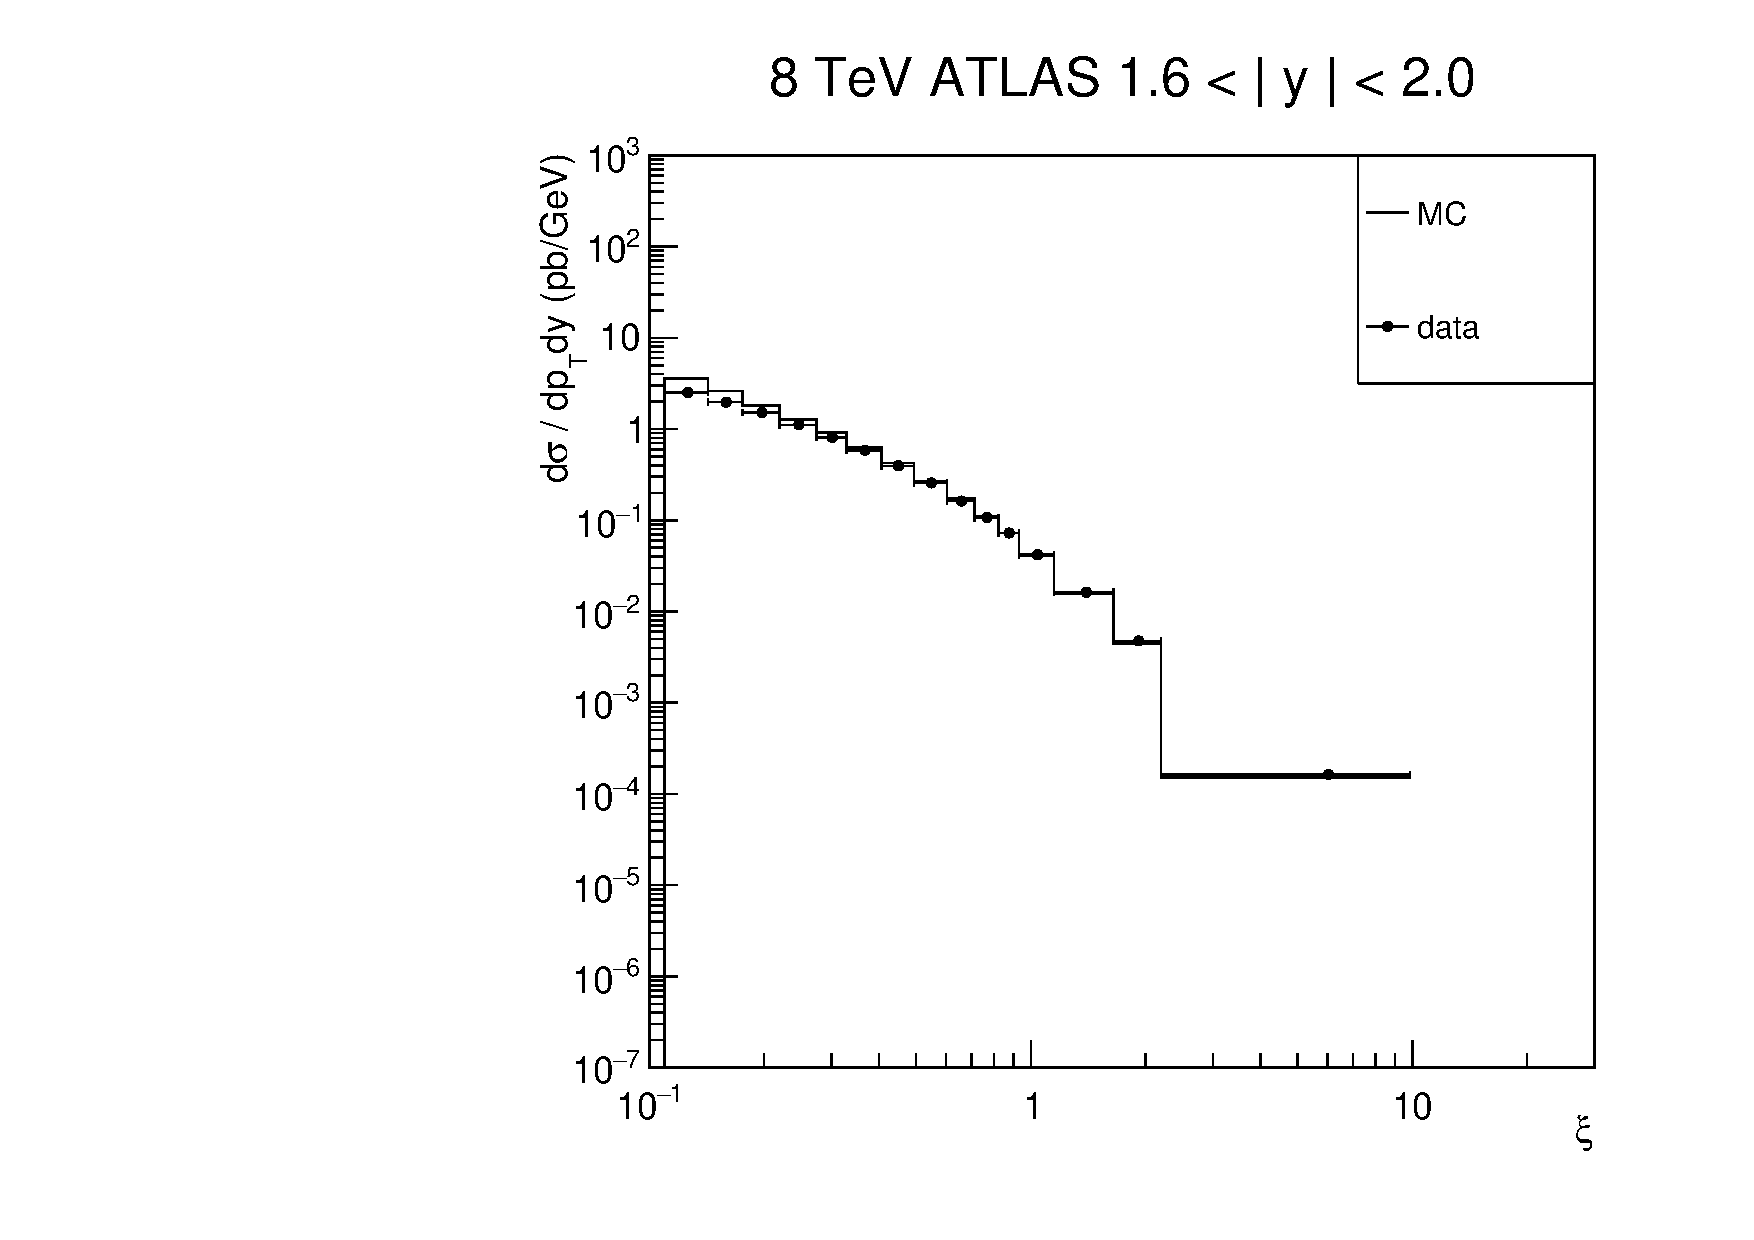
\includegraphics[width = 0.4\textwidth]{xi_8_A_y5.pdf}
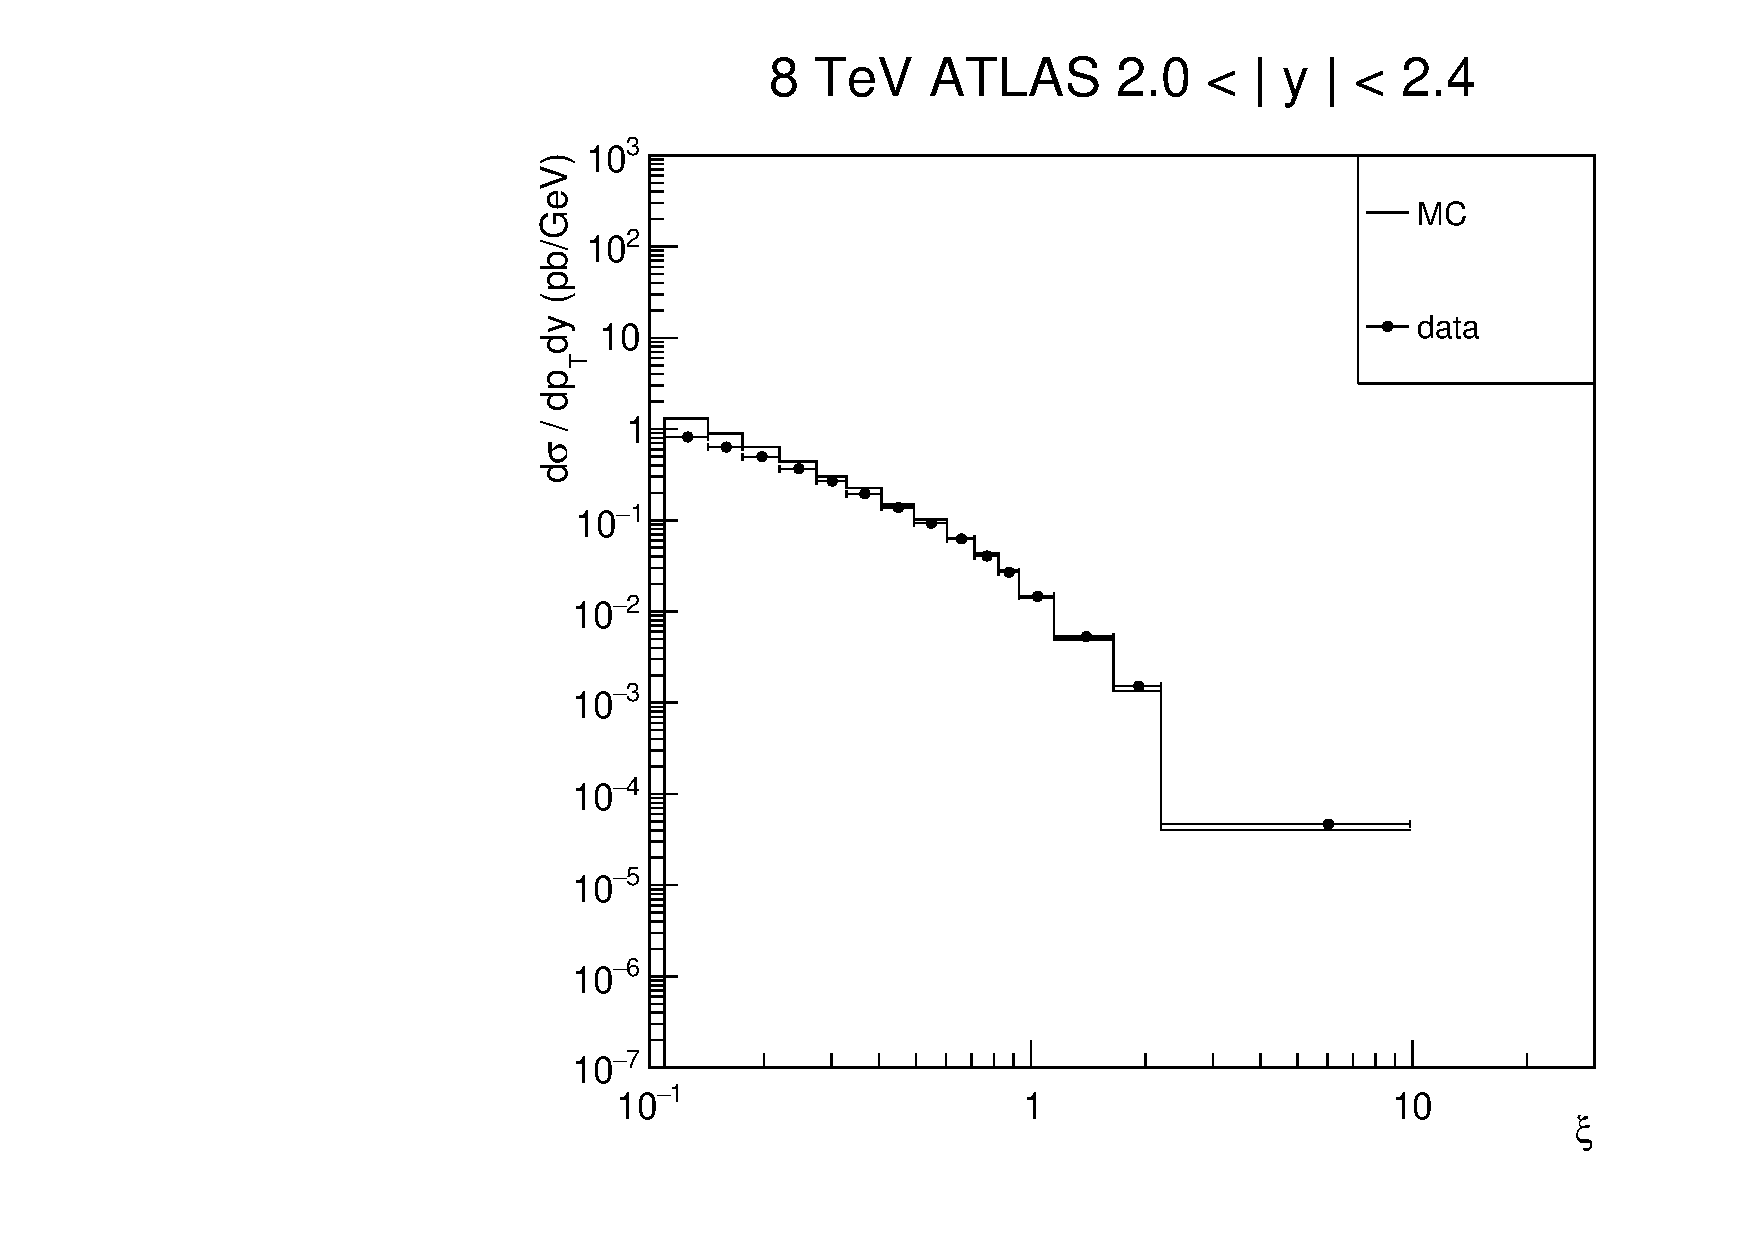
\includegraphics[width = 0.4\textwidth]{xi_8_A_y6.pdf}
%\caption{Comparison between MC $\xi$ distribution and data points in the six $y$ bins of the data, for 8 TeV. All histograms divided by total nr events and multiplied by same normalization factor. Data is not scaled.}\label{f:xi_comp}
\end{figure}

\clearpage

\begin{figure}[h!]
\centering
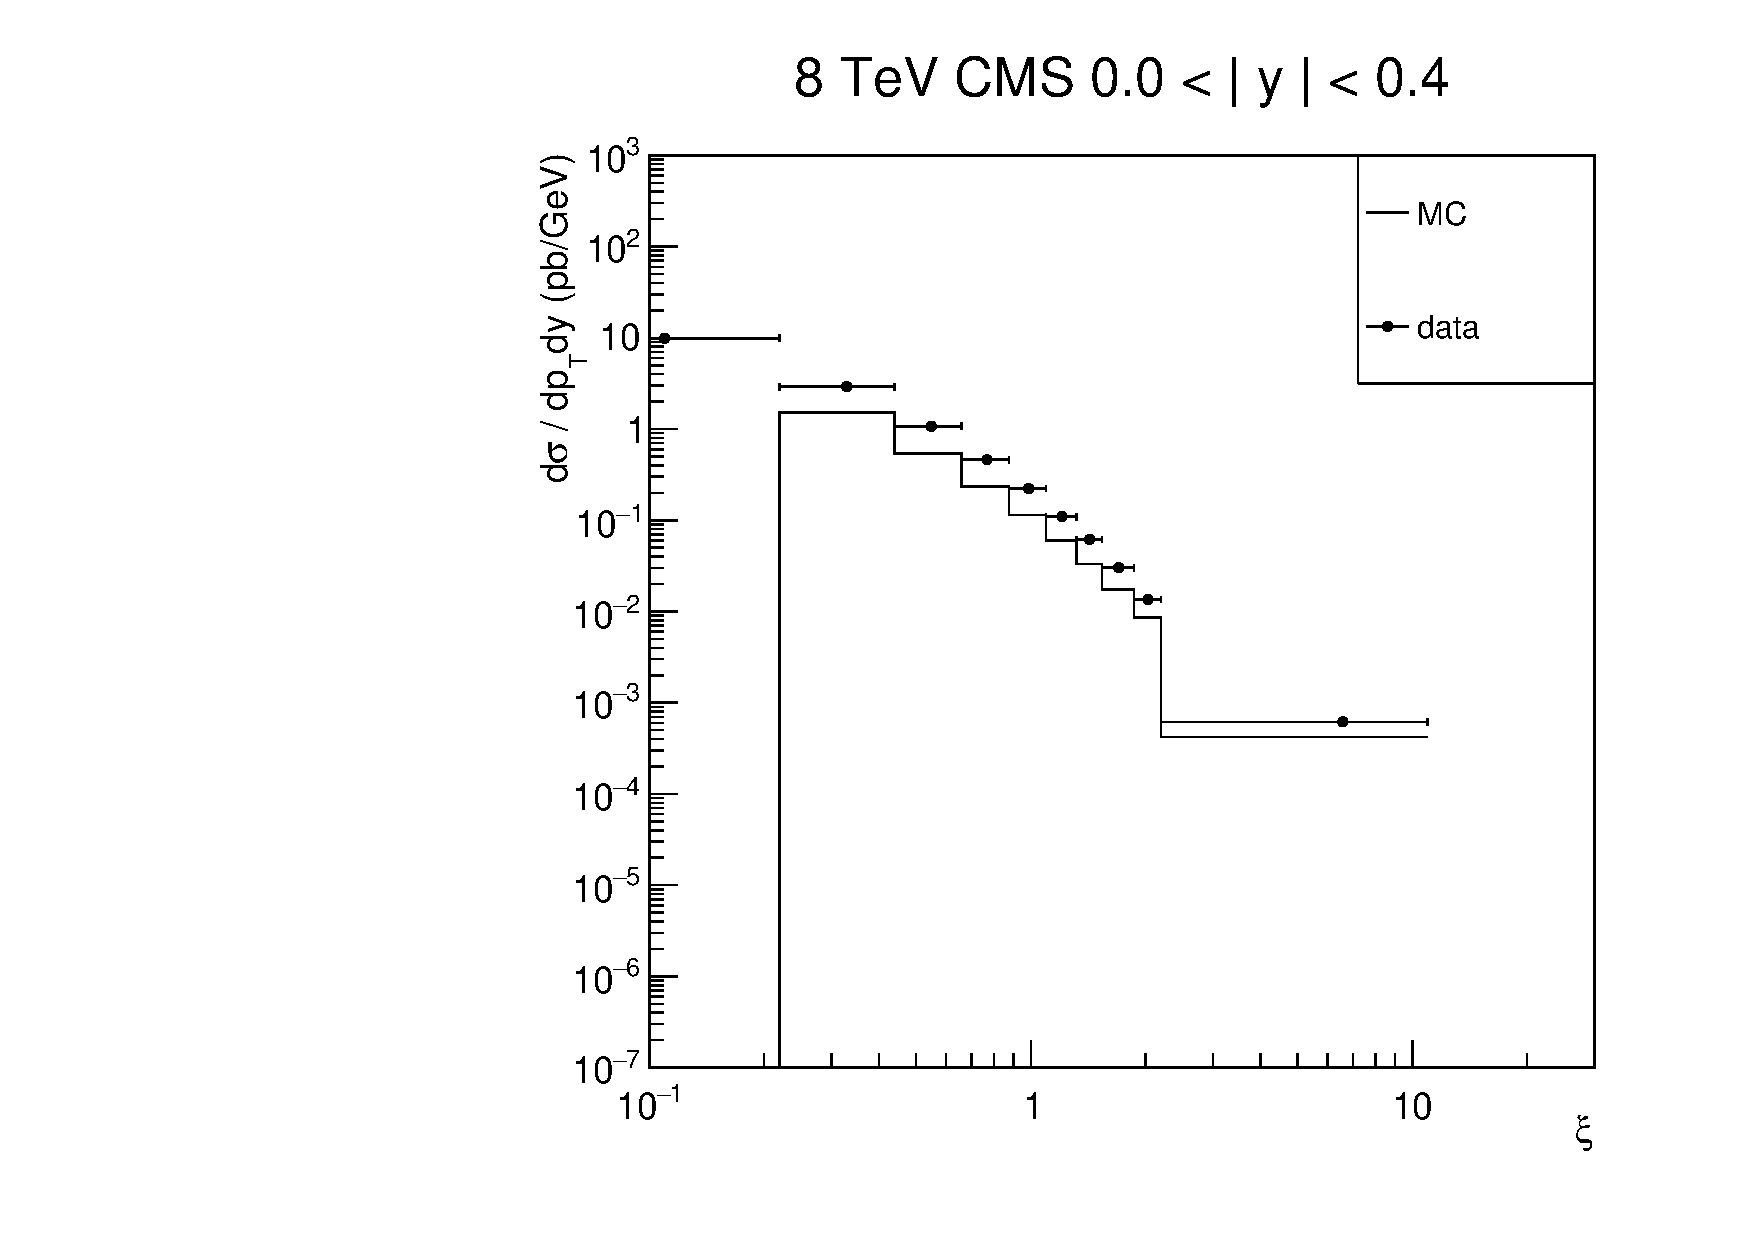
\includegraphics[width = 0.4\textwidth]{xi_8_C_y1.pdf}
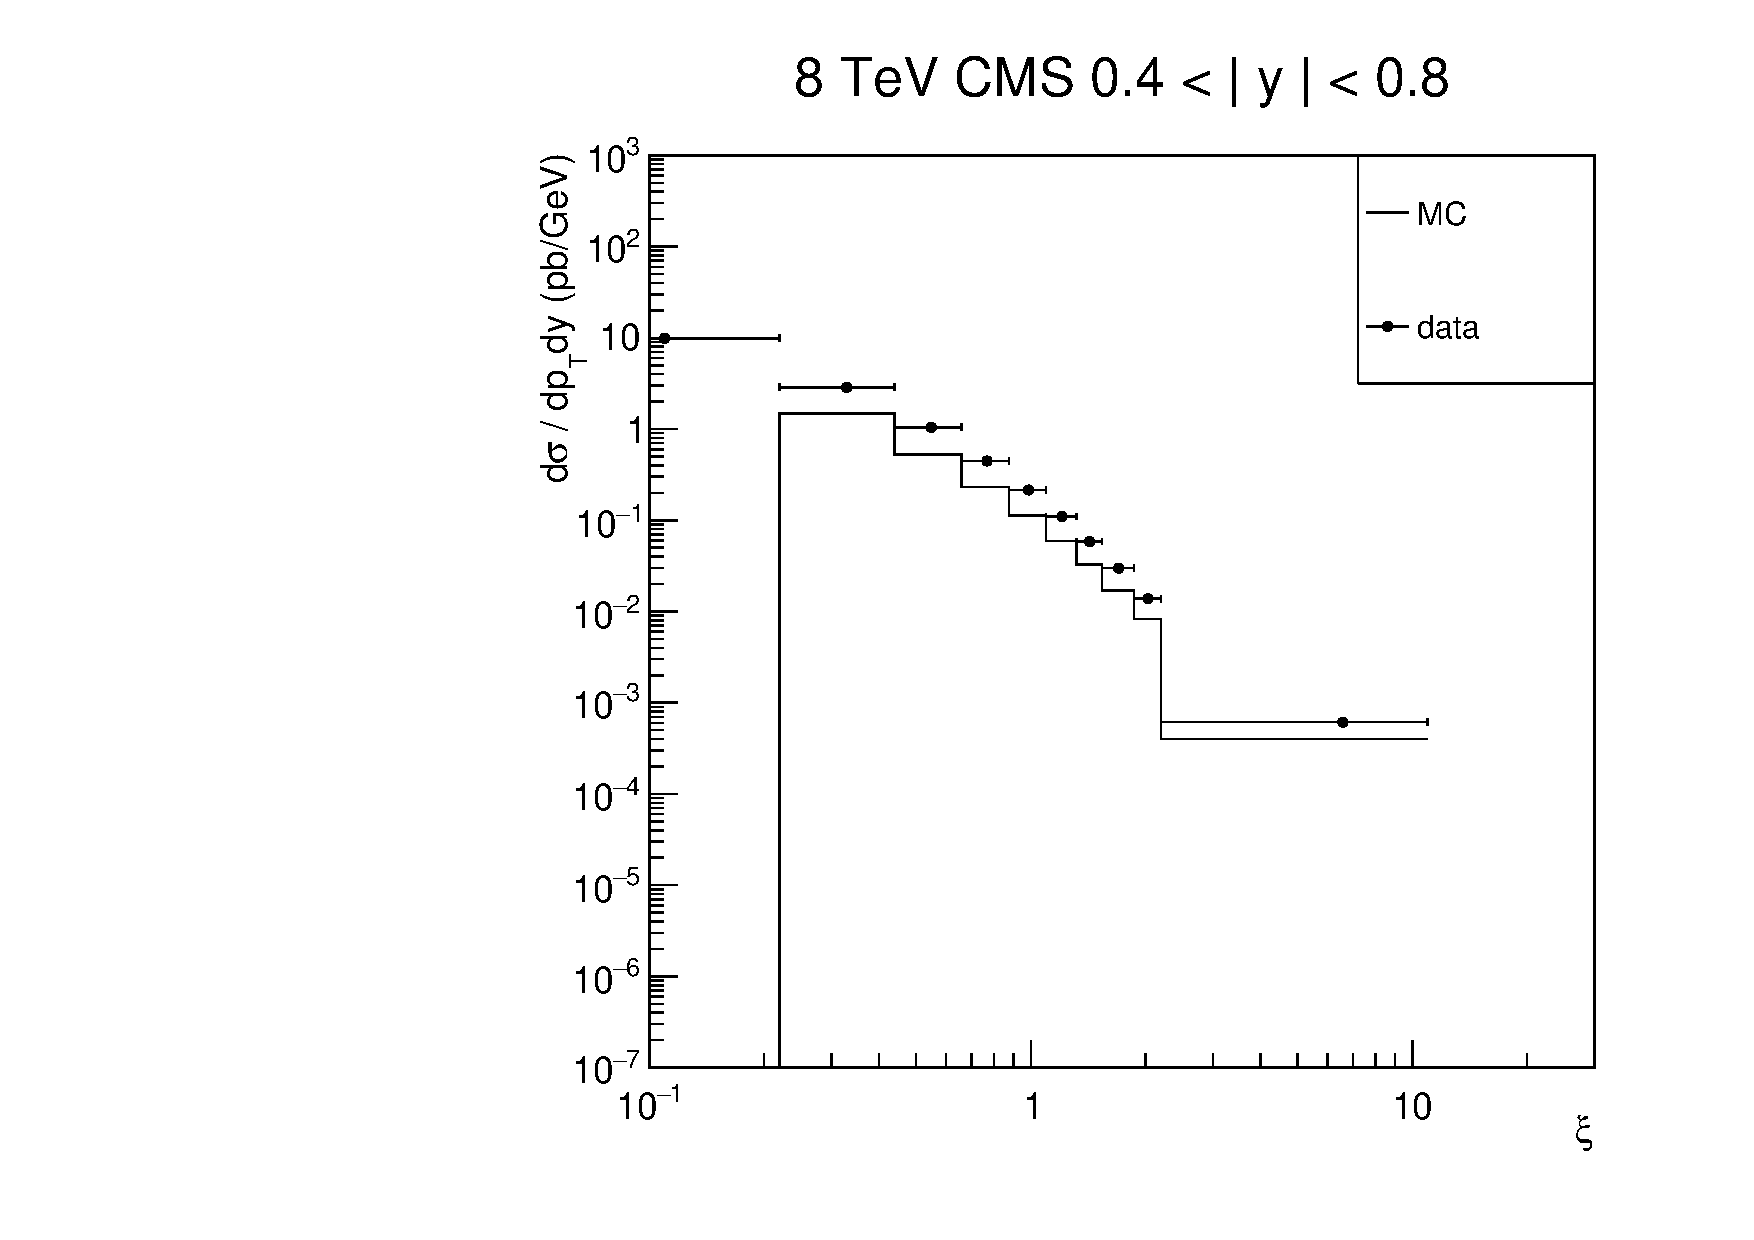
\includegraphics[width = 0.4\textwidth]{xi_8_C_y2.pdf}

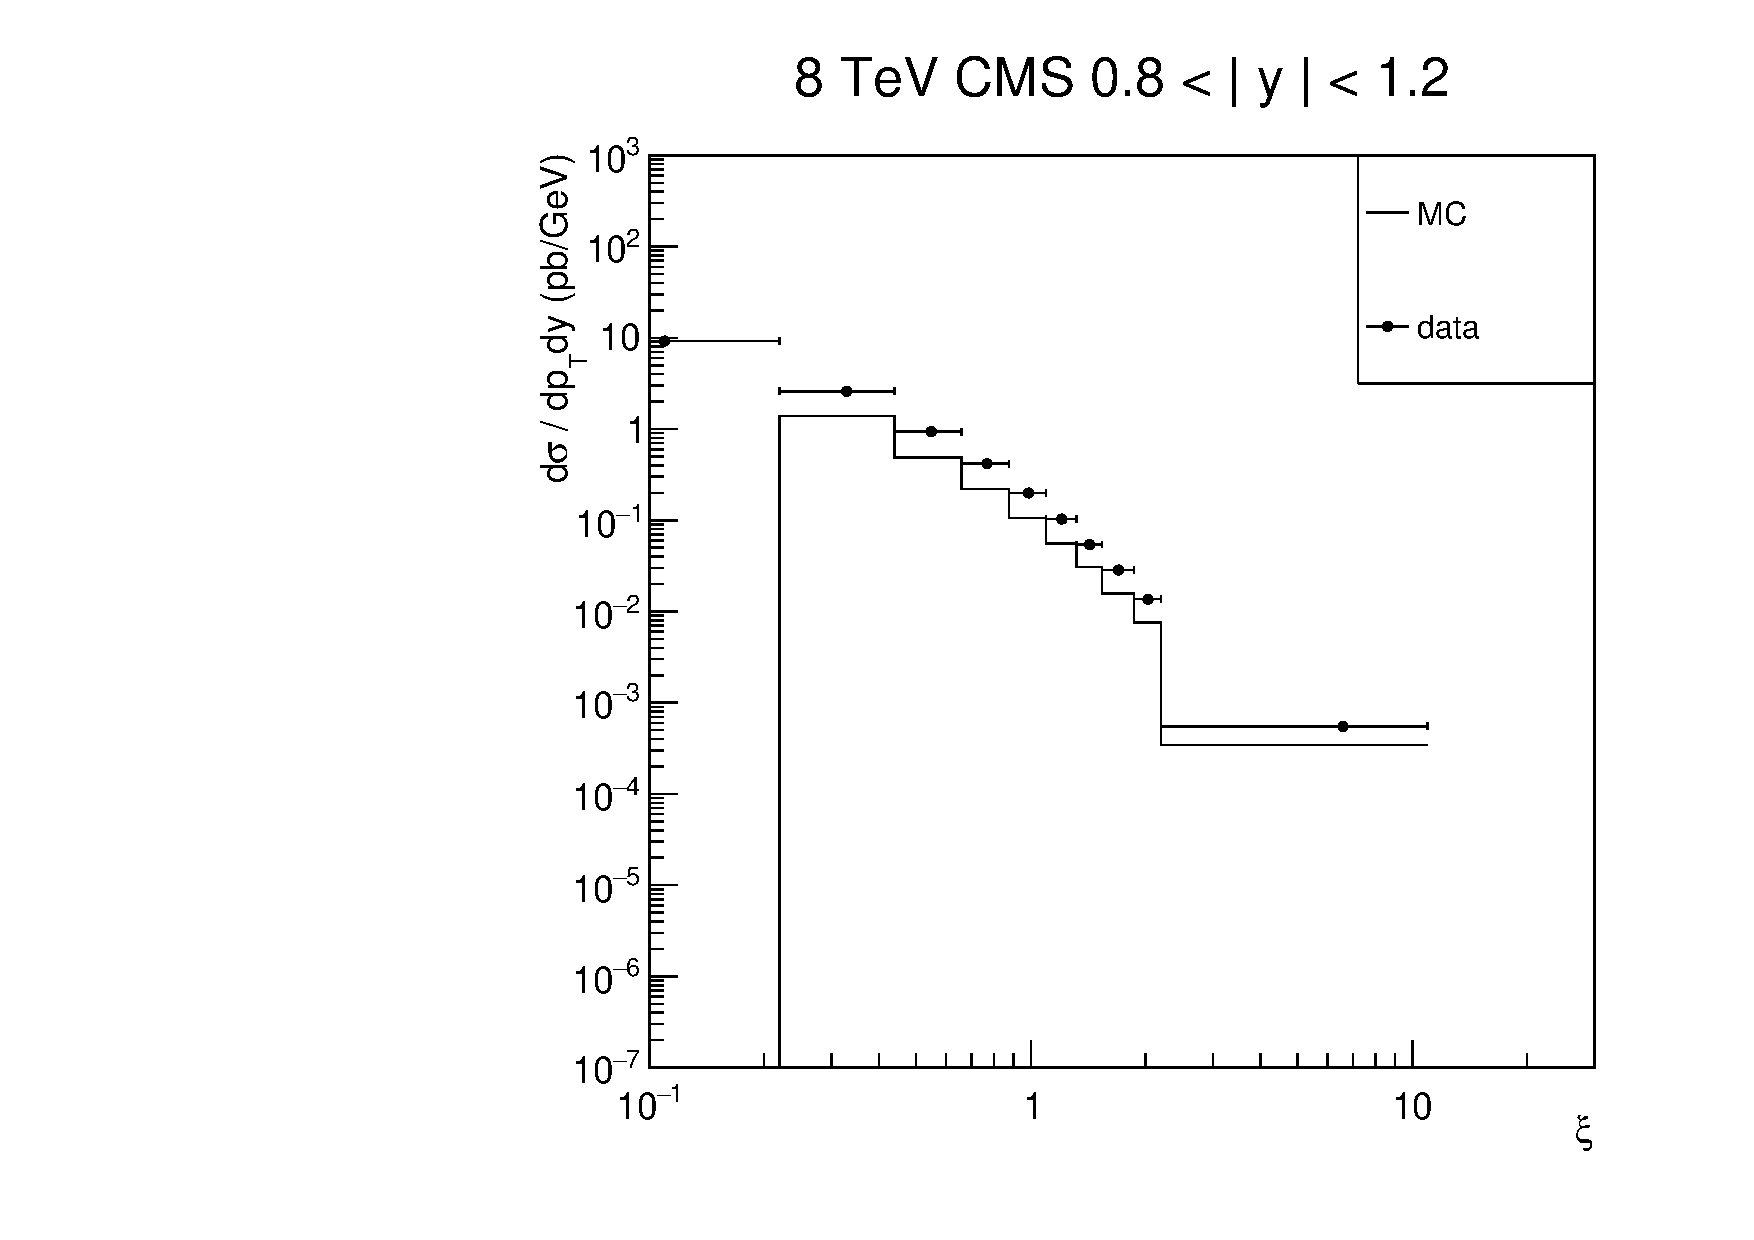
\includegraphics[width = 0.4\textwidth]{xi_8_C_y3.pdf}
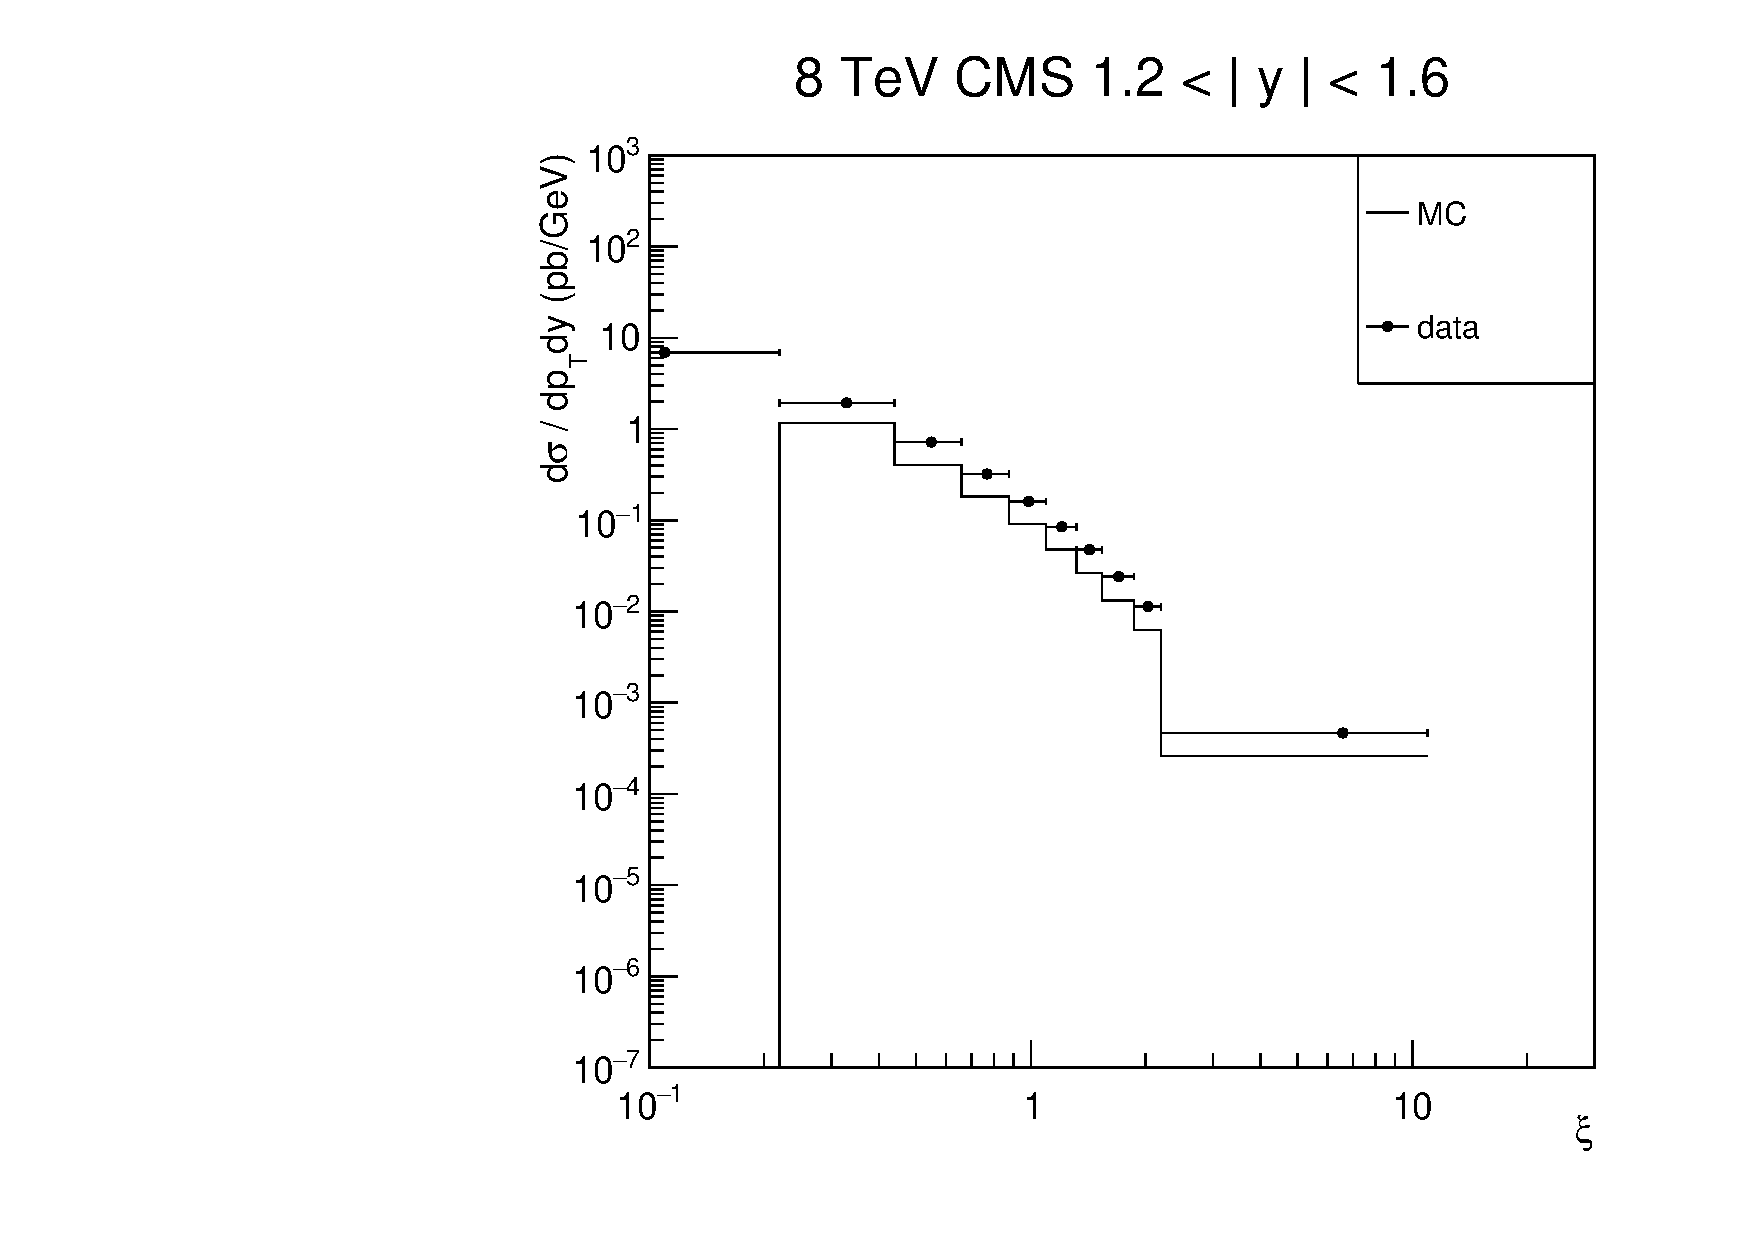
\includegraphics[width = 0.4\textwidth]{xi_8_C_y4.pdf}

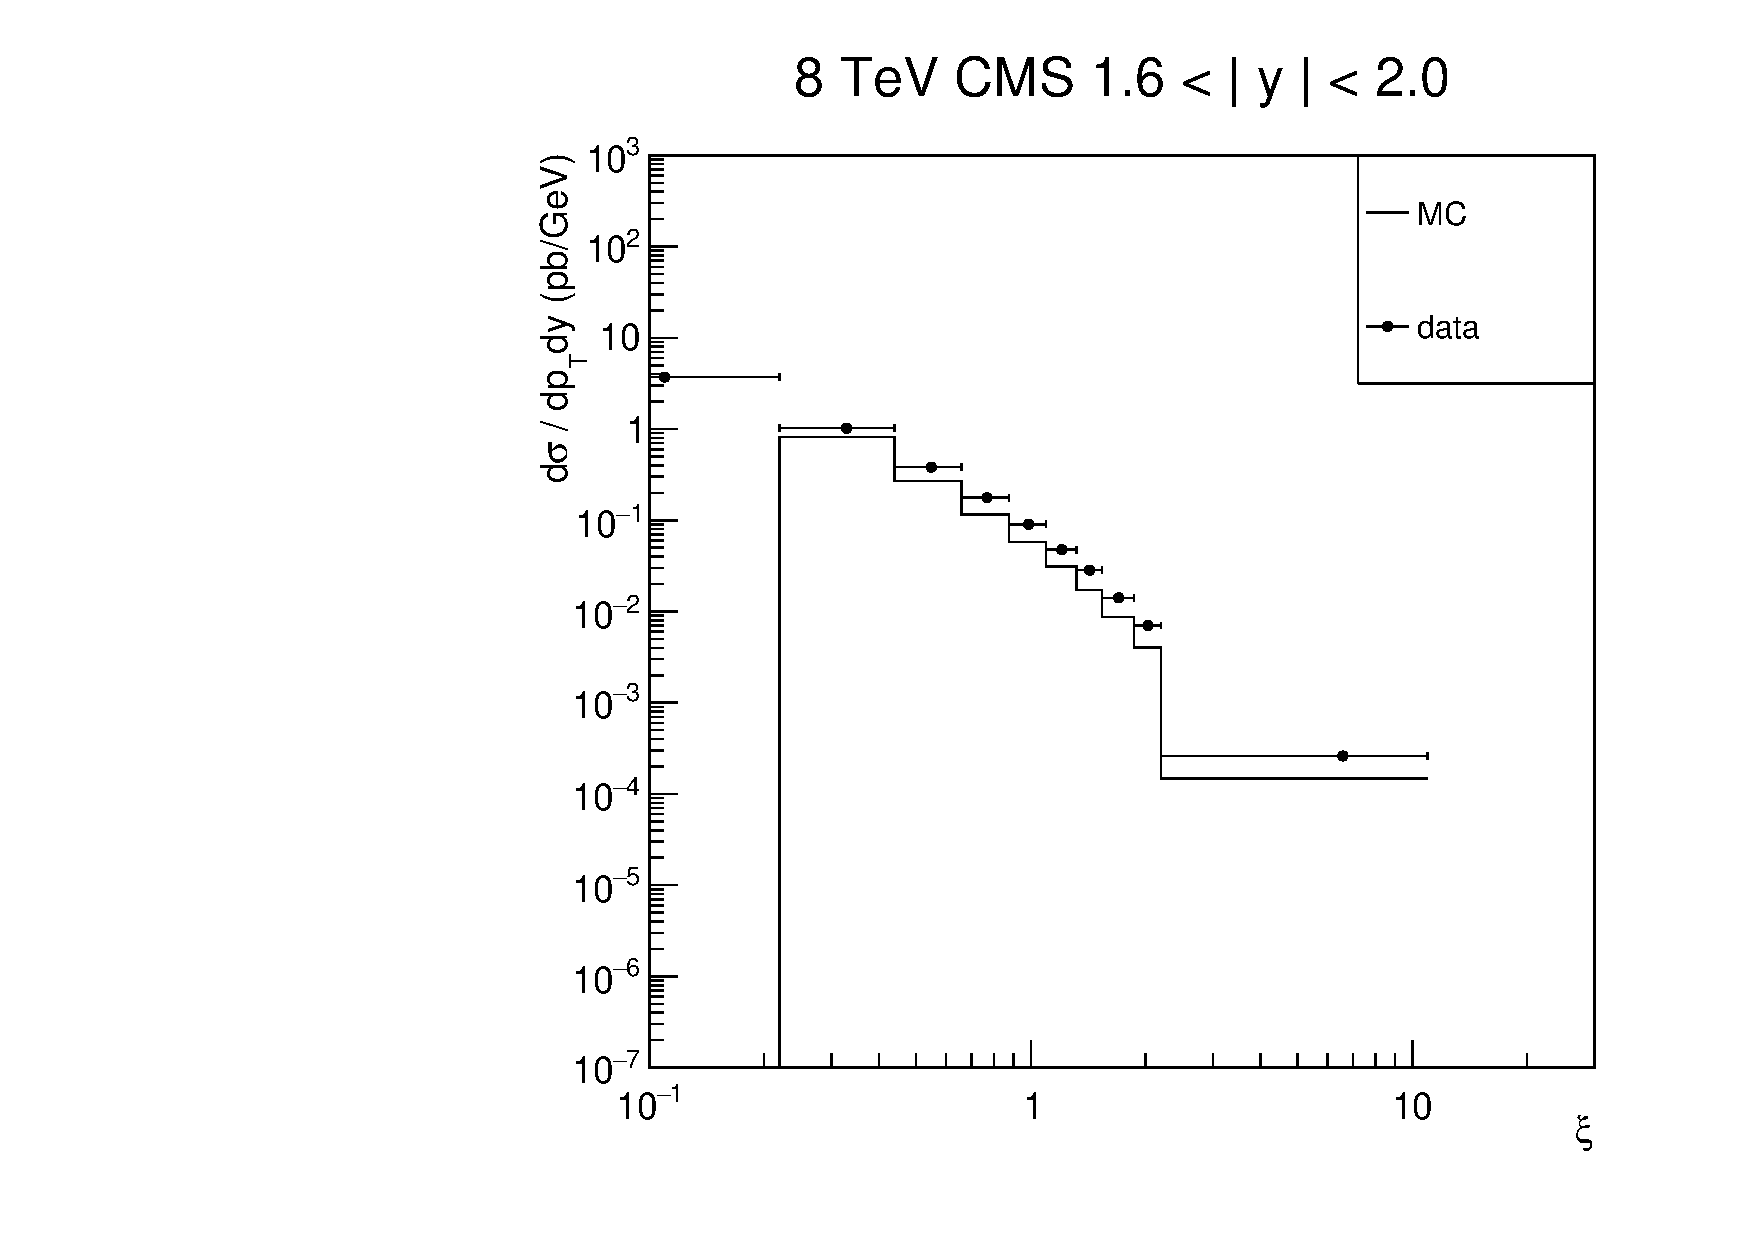
\includegraphics[width = 0.4\textwidth]{xi_8_C_y5.pdf}
%\caption{Comparison between MC $\xi$ distribution and data points in the six $y$ bins of the data, for 8 TeV. All histograms divided by total nr events and multiplied by same normalization factor. Data is not scaled.}\label{f:xi_comp}
\end{figure}

\clearpage

\begin{figure}[h!]
\centering
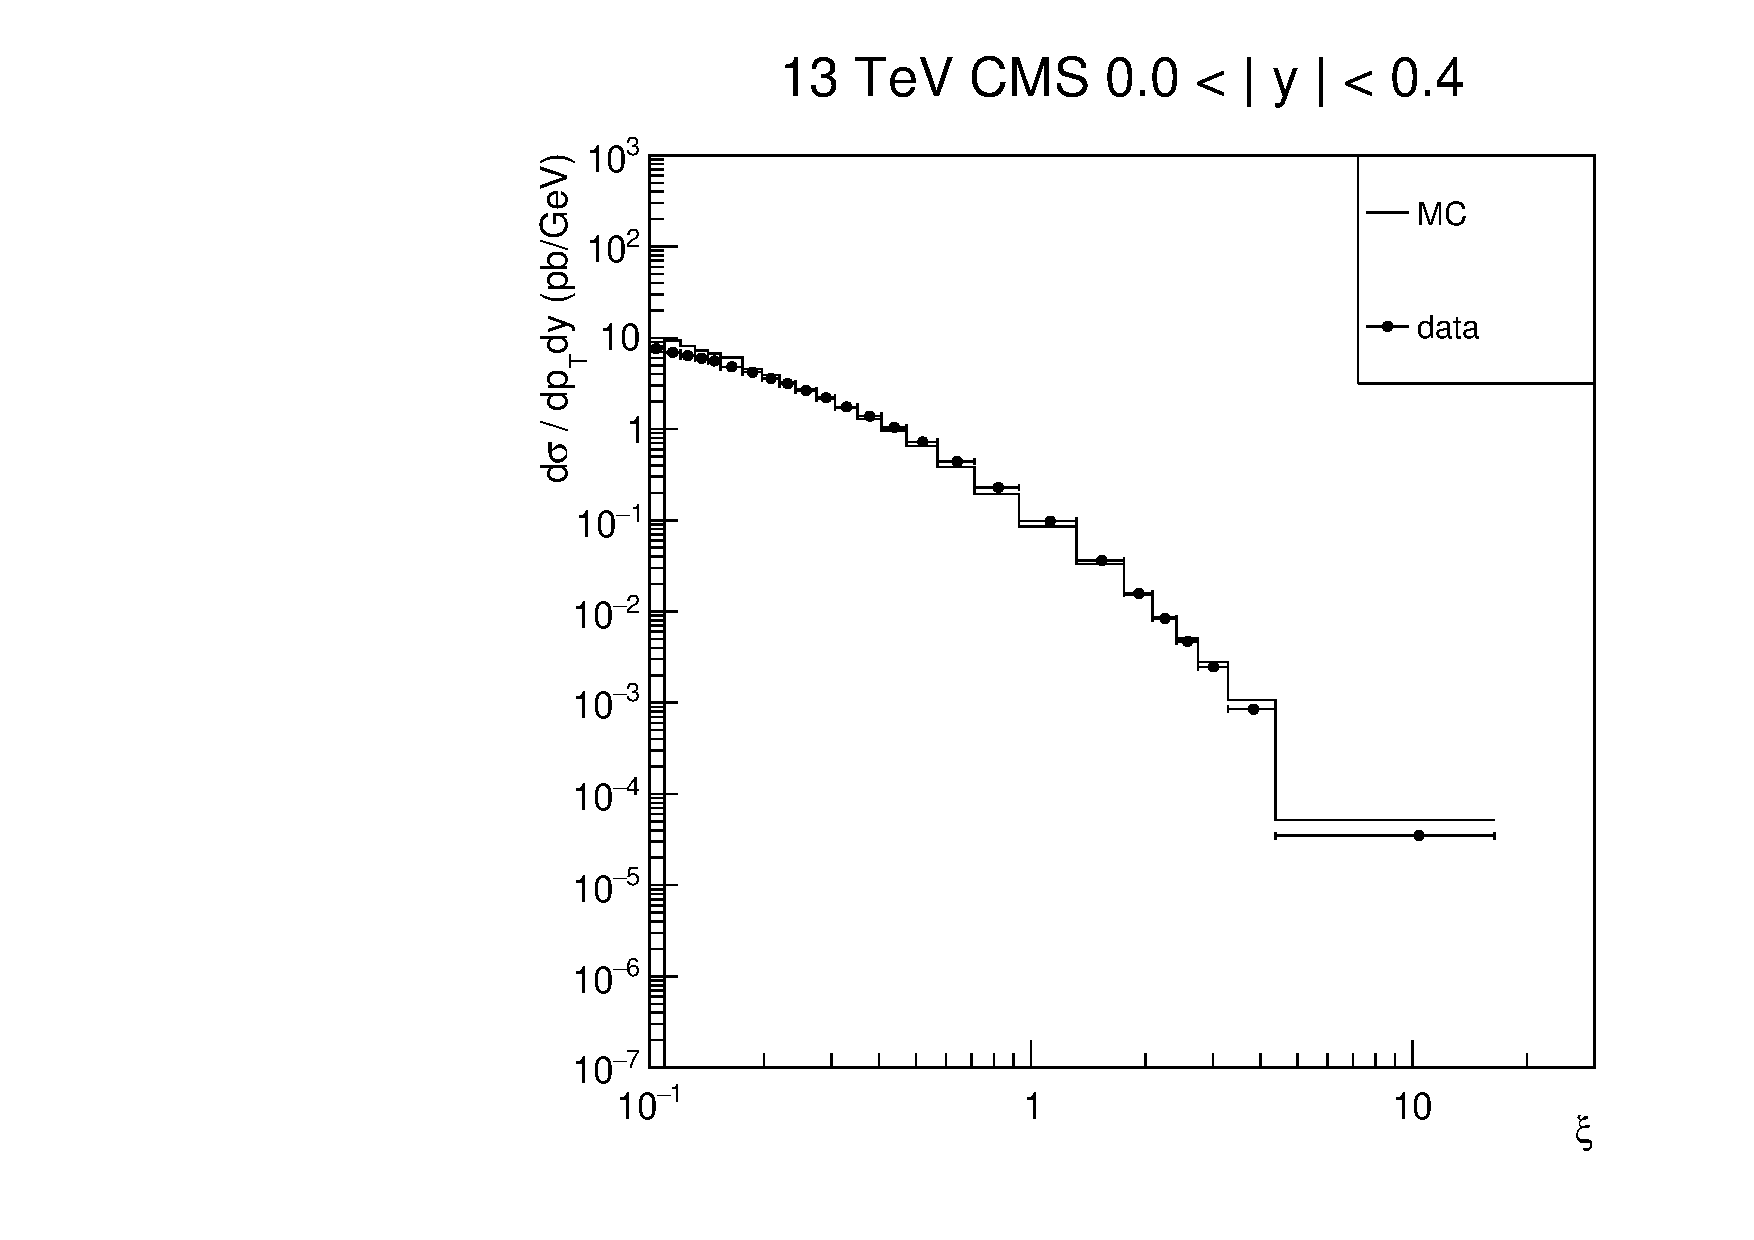
\includegraphics[width = 0.4\textwidth]{xi_13_C_y1.pdf}
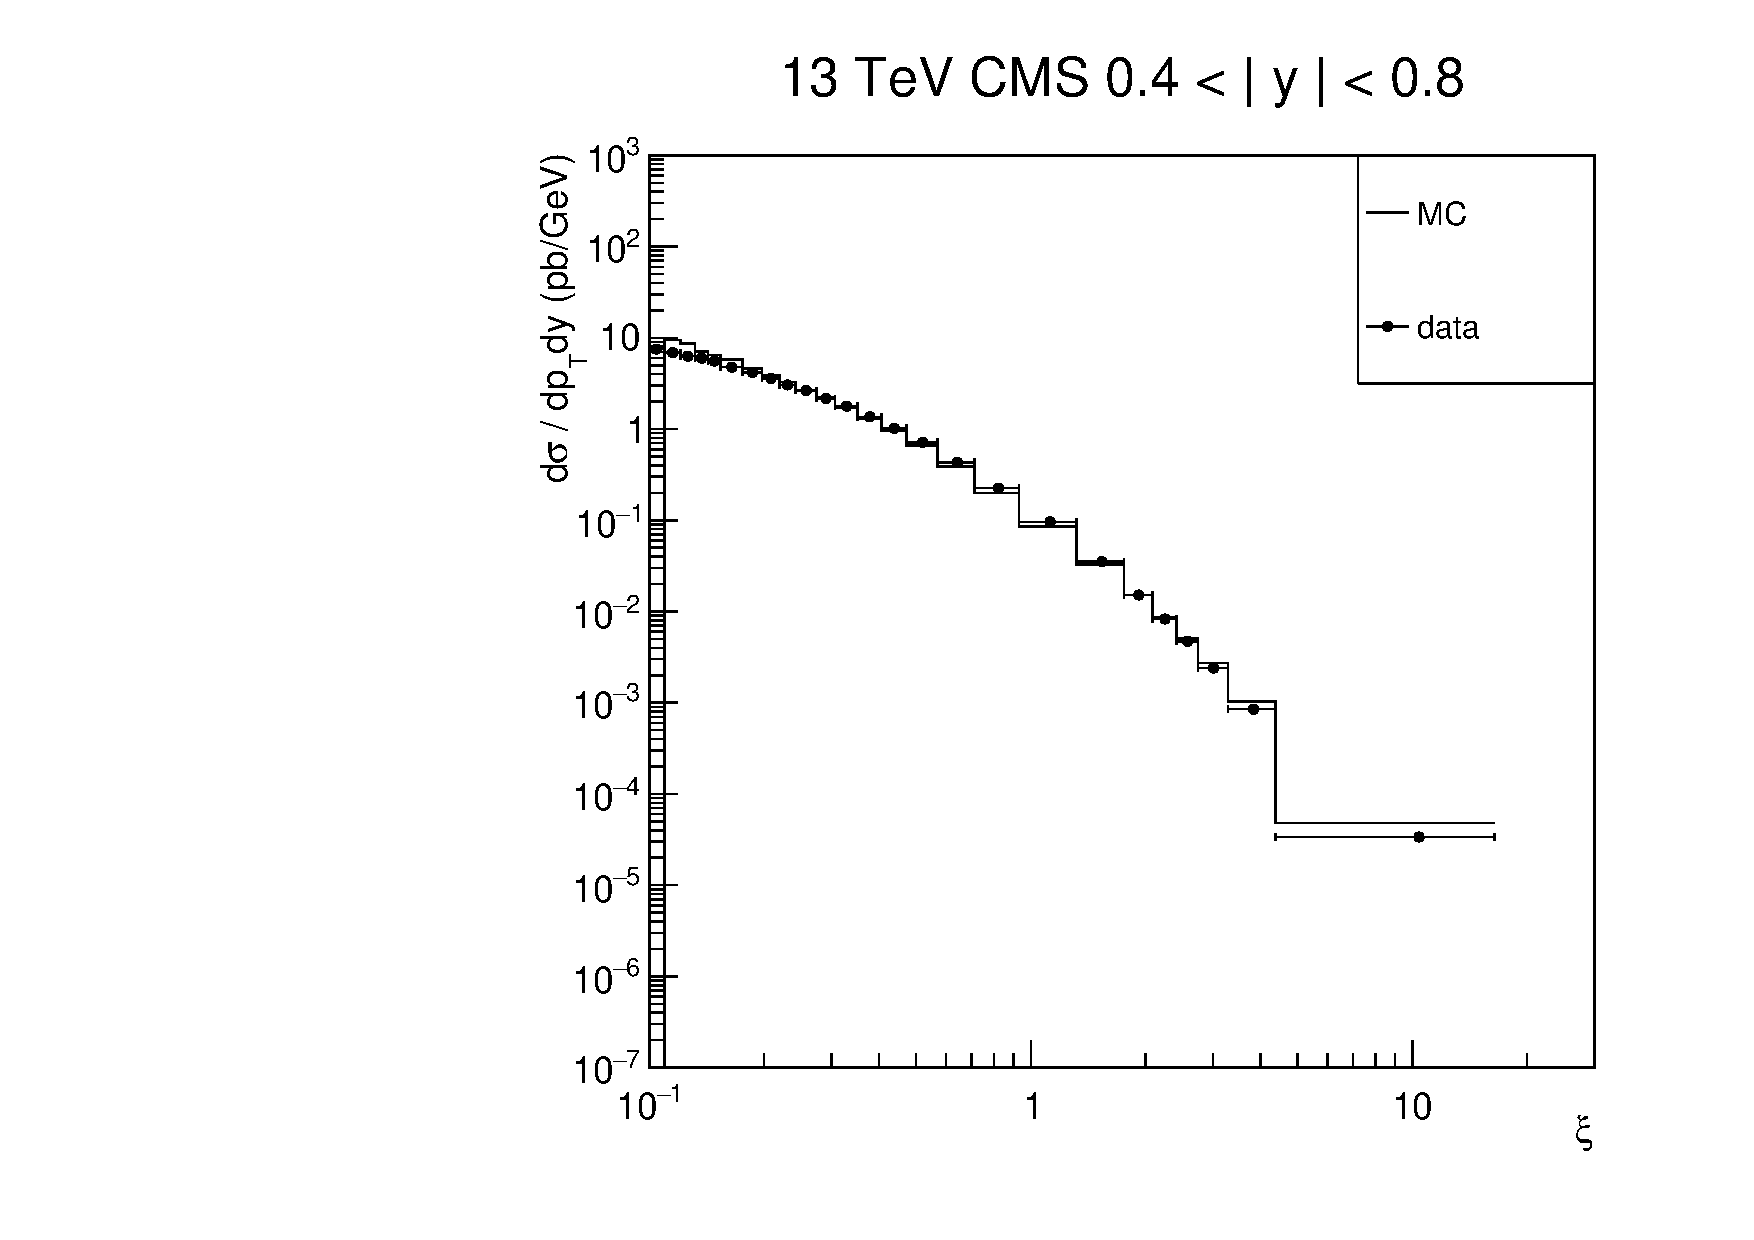
\includegraphics[width = 0.4\textwidth]{xi_13_C_y2.pdf}

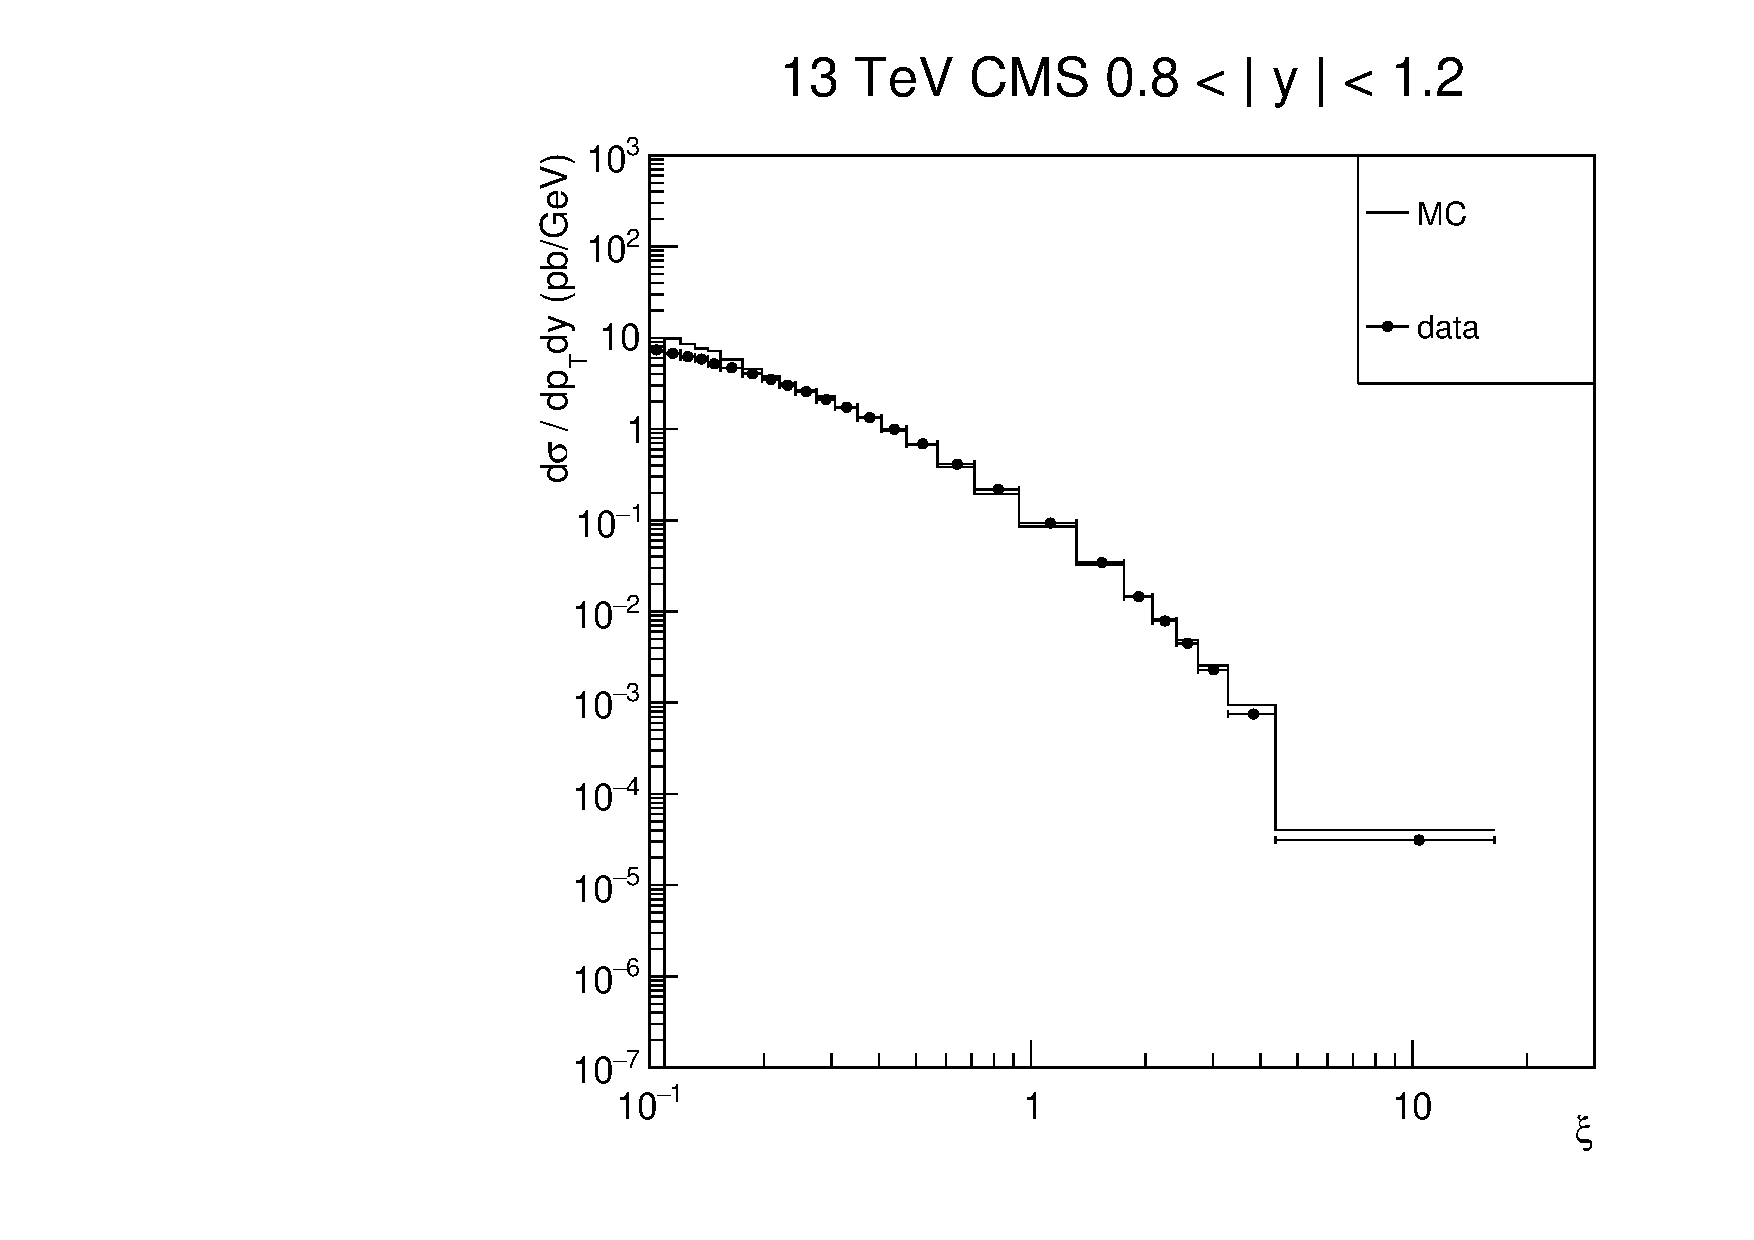
\includegraphics[width = 0.4\textwidth]{xi_13_C_y3.pdf}
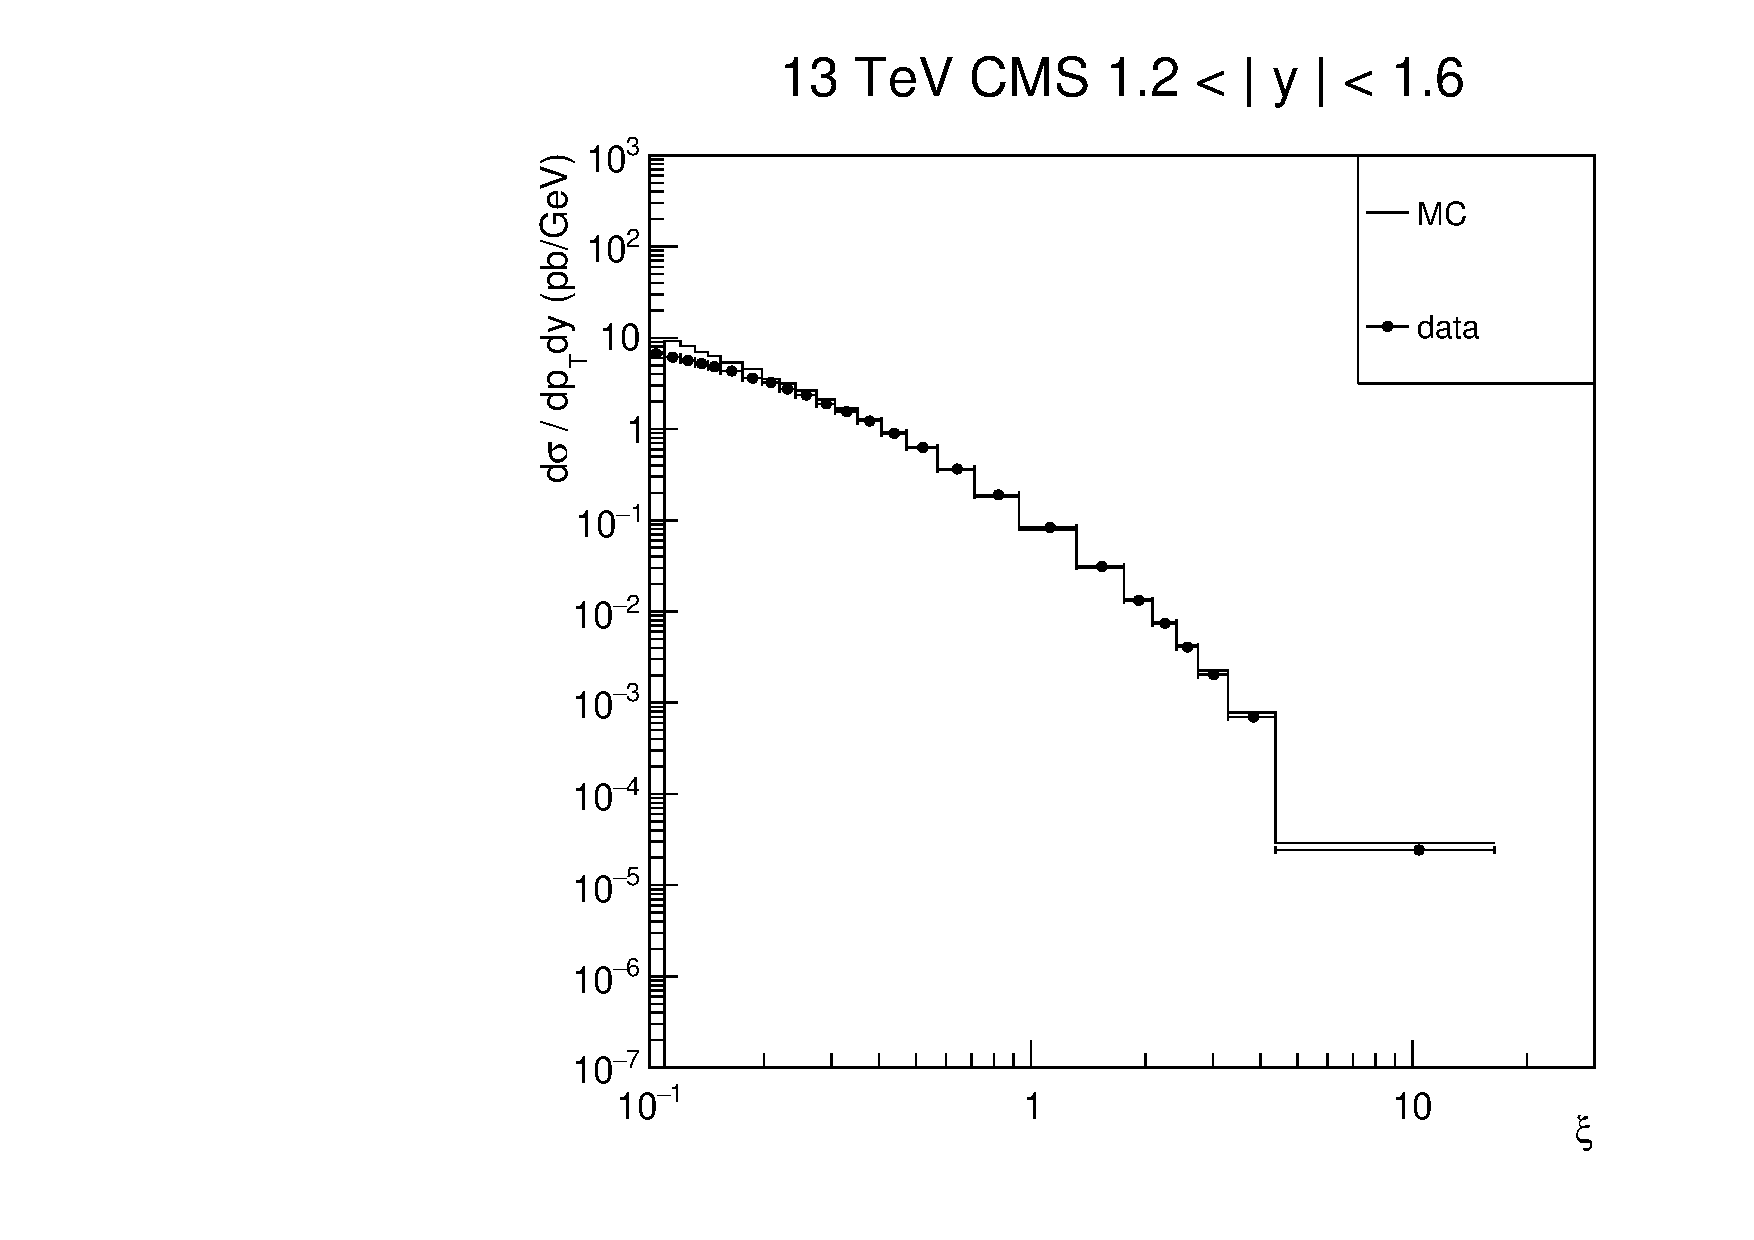
\includegraphics[width = 0.4\textwidth]{xi_13_C_y4.pdf}

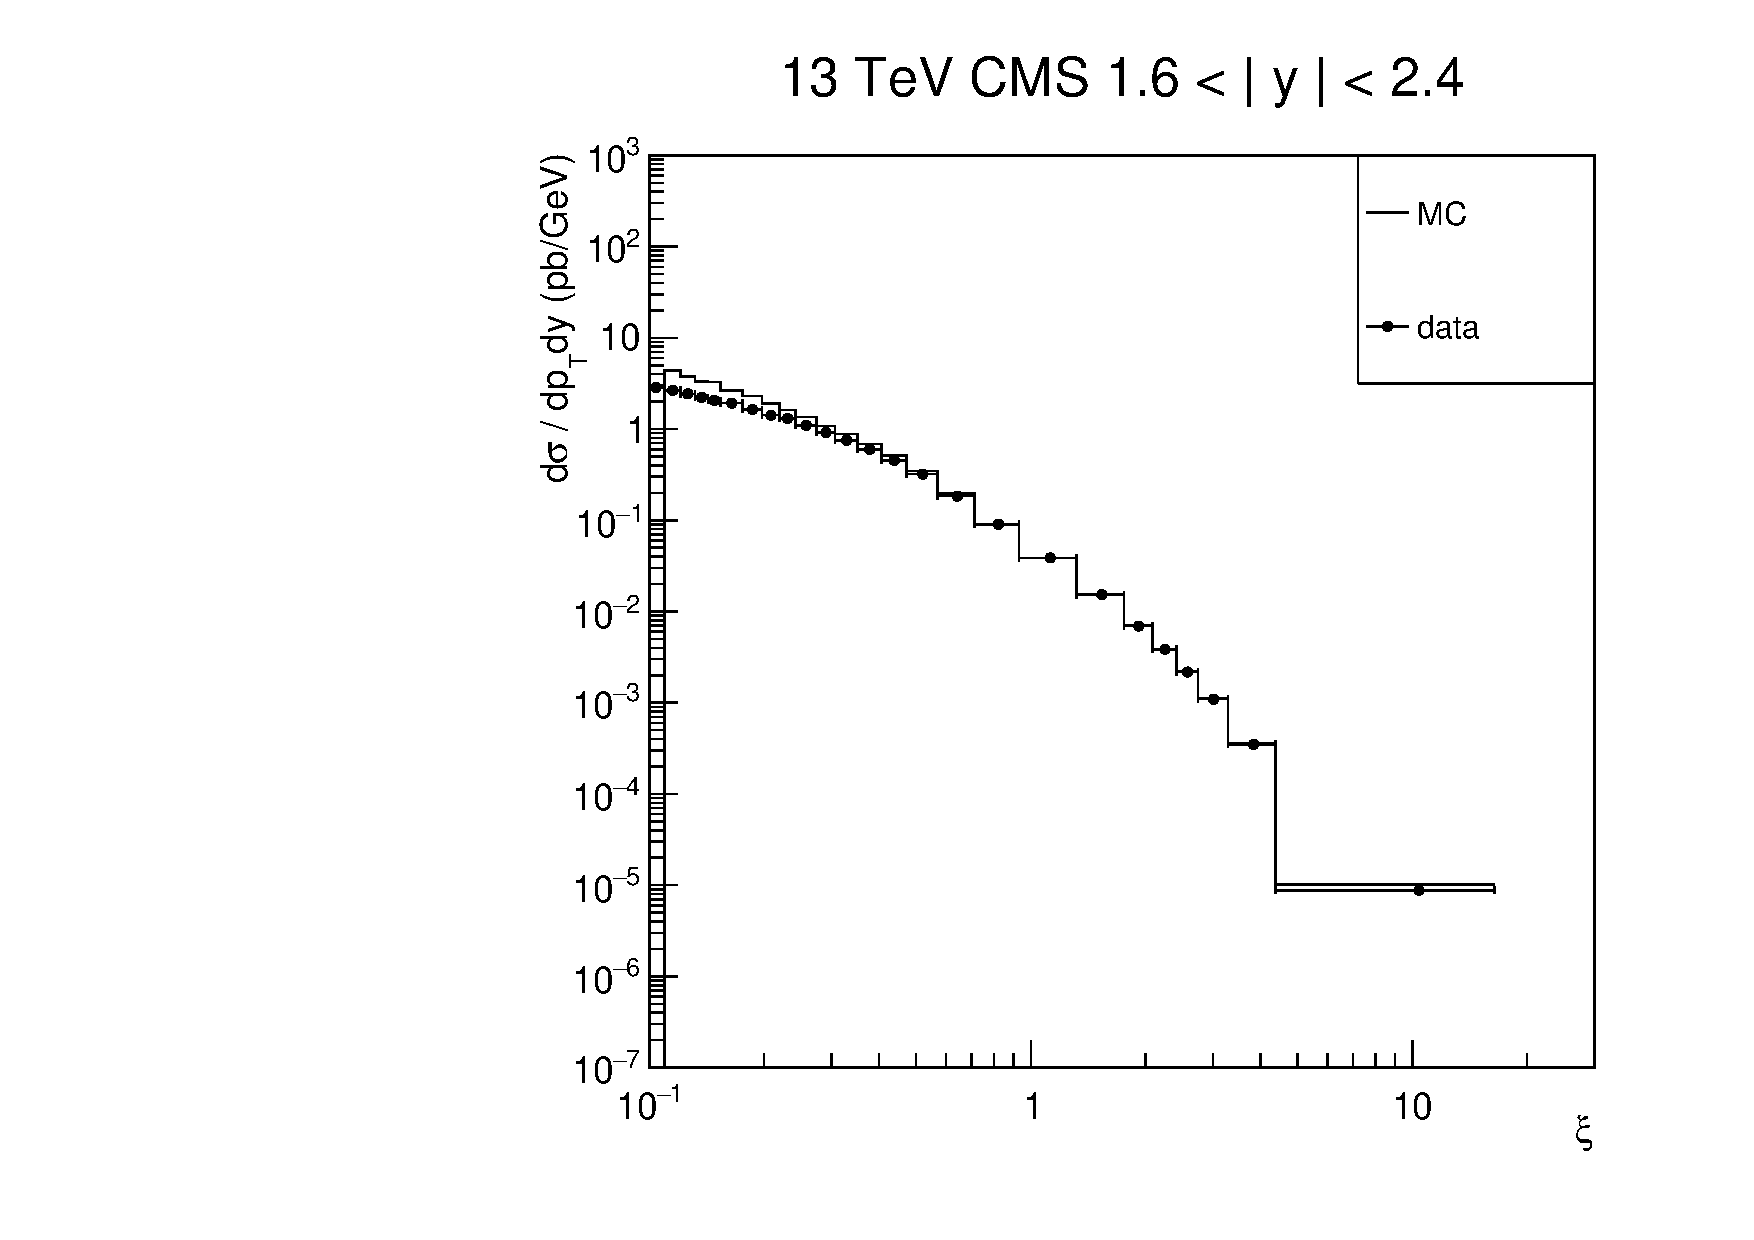
\includegraphics[width = 0.4\textwidth]{xi_13_C_y5.pdf}
%\caption{Comparison between MC $\xi$ distribution and data points in the six $y$ bins of the data, for 8 TeV. All histograms divided by total nr events and multiplied by same normalization factor. Data is not scaled.}\label{f:xi_comp}
\end{figure}

\end{document}